% vim: se spl=fr:
%===============================================================================
\documentclass[aspectratio=43]{beamer} %handout 16:10 16:9 14:9 5:4 4:3(d) 3:2
\usetheme[webtitle=false]{LACLsb}
\setbeamertemplate{navigation symbols}{}
%===============================================================================
%\usepackage{amsfonts}
\usepackage{amsmath}
\usepackage{amssymb}
\usepackage{array}
\usepackage[french]{babel}
\usepackage{booktabs}
\usepackage[T1]{fontenc}
\usepackage{graphicx}
\usepackage[utf8]{inputenc}
\usepackage{tabu}
\usepackage{tikz}
\usepackage{xcolor}
\usepackage{xspace}
\usepackage{libertine}
\usepackage{hyperref}
%===============================================================================
%\usetikzlibrary{automata,calc,shapes,mindmap,shadows}
\usetikzlibrary{automata,shadows}
\hypersetup{%
  linktoc=all,
  breaklinks,
  colorlinks,
  linkcolor=,
  citecolor=vert,
  urlcolor=blue,
  baseurl       = http://,
  pdfcreator    = {\LaTeX{}},
  pdfauthor     = {Quentin MONNET},
  pdftitle      = {Modèles et mécanismes pour la protection contre les attaques par déni de service dans les réseaux de capteurs sans fils},
  pdfsubject    = {Soutenance de thèse},
  pdfkeywords   = {Université Paris-Est; Soutenance de thèse; Sécurité; Réseaux de capteurs; Communications sans fil; Déni de service; Théorie des jeux}
}
%===============================================================================
\definecolor{vert}{rgb}{0.11,0.47,0.11}
%===============================================================================
\newcommand\apriori{\textit{a~priori}\xspace}
\newcommand\aposteriori{\textit{a~posteriori}\xspace}
\newcommand\defacto{\textit{de~facto}\xspace}
\newcommand\eg{\textit{e.g.}\xspace}
\newcommand\ie{\textit{i.e.}\xspace}
\newcommand\via{\textit{via}\xspace}
\newcommand\etc{\textit{et~cætera}\xspace}
\newcommand\Wsns{Wireless sensor networks\xspace}
\newcommand\wsns{wireless sensor networks\xspace}
\newcommand\Wsn{Wireless sensor network\xspace}
\newcommand\wsn{wireless sensor network\xspace}
\newcommand\dos{denial of service\xspace}
\newcommand\bs{base station\xspace}
\newcommand\BS{BS\xspace}
\newcommand\ch{cluster head\xspace}
\newcommand\chs{cluster heads\xspace}
\newcommand\CH{CH\xspace}
\newcommand\CHs{CHs\xspace}
\newcommand\leach{\textit{LEACH}\xspace}
\newcommand\cn{\textit{cNode}\xspace}
\newcommand\cns{\textit{cNodes}\xspace}
\newcommand\cnsns{\textit{cNodes}}
\newcommand\vn{\textit{vNode}\xspace}
\newcommand\vns{\textit{vNodes}\xspace}
\newcommand\ns{\textsf{ns-3}\xspace}
\newcommand\todo[1]{\textcolor{red}{\textbf{TO DO: }#1}}
\newenvironment{colorblock}[1][yellow]{\setbeamercolor{structure}{fg=#1}\setbeamercolor{block title}{use=structure,fg=black,bg=structure.fg!60!white}\setbeamercolor{block body}{parent=normal text,use=block title,bg=block title.bg!40!bg}\setbeamercolor{item projected}{fg=block title.fg}}{}
%===============================================================================
\def\thetitle{Modèles et mécanismes pour la protection\\contre les attaques par déni de service\\dans les réseaux de capteurs sans fil}

\def\theauthor{{\scriptsize Soutenance de thèse de}\\{\large Quentin~\textsc{Monnet}}\\\smallskip{\scriptsize Directrice~:}\\{\small Prof.~Lynda~\textsc{Mokdad}}}

\def\thedate{\small Vendredi 17 juillet 2015}

\title[Déni de service et réseaux de capteurs]{\thetitle}
\author[Qu.~\textsc{Monnet}]{\theauthor}
\date[Soutenance de thèse --- 17 juillet 2015]{\thedate}

%\institute{\includegraphics[width=.3\textwidth]{UPE_marron.png}}
%===============================================================================
%===============================================================================
\begin{document}
%===============================================================================
%\begin{frame}
  %\titlepage
%\end{frame}
%===============================================================================
\bgroup
\setbeamercolor{background canvas}{bg=blueLACL}
\setbeamercolor{normal text}{fg=red}
\begin{frame}[plain]{}
  \advance\textwidth-2.5\baselineskip
  \hsize\textwidth
  \columnwidth\textwidth

  \vspace{\baselineskip}\hspace{-.5em}%
  \begin{minipage}[c][.9\textheight]{\textwidth}
    \color{white}
    \center
    \theauthor\par\vfill
    \hrule
    \medskip
    \Large\thetitle\par\medskip
    \hrule\vfill
    \thedate\par\vfill
    
\includegraphics[width=.3\textwidth]{upe.png}
  \end{minipage}
\end{frame}
\egroup
%===============================================================================
\begin{frame}{Présentation}
  % \setcounter{tocdepth}{1}
  \tableofcontents[sectionstyle=show,subsectionstyle=show]
\end{frame}
%===============================================================================
\section[Contexte]{Réseaux de capteurs et déni de service}
%===============================================================================
\begin{frame}{Capteurs}
  \alert{Capteurs} (ou \textit{nœuds}) {\footnotesize(anglais: \textit{sensors, nodes, motes})}: de petits appareils
  \begin{itemize}
    \item effectuant des \alert{mesures} (lumière, CO$_\text{2}$, température, champ magnétique, vibrations, \dots)
    \item communiquant \alert{sans fil (\textit{ad-hoc})}
    \item reliés à une \alert{station de base}
  \end{itemize}
  \begin{minipage}[c]{0.5\textwidth}
    \begin{block}{Ressources limitées}
      \begin{itemize}
        \item Faibles capacités de \alert{calcul}
        \item Peu de \alert{mémoire} disponible
        \item \alert{Énergie} limitée (batterie)
      \end{itemize}
    \end{block}
  \end{minipage}
  \hfill
  \begin{minipage}[c]{0.42\textwidth}
    \centering
    \fontsize{6}{8}\selectfont
    \begin{tikzpicture}[%
        scale=.4,
        sensor/.style={ circle, minimum size=3cm, very thick, draw=black!50, fill=black!20 },%
        module/.style={ rounded corners, text width=6em, minimum height=6em, align=center, very thick, draw=black!50, top color=white, bottom color=black!20, inner sep=0pt }%
      ]
      \node (sensor) at (   0, -0.1) [sensor]{\footnotesize Capteur};
      \draw [rounded corners=3pt,top color=black!20,draw=black!50,very thick] (-2,3)--(-2,5)--(-2.5,5)--(-2.5,3)--cycle ;
      \node (mesure) at ( 2.2, 2) [module]{Unit\'e de captage\\(mesures physiques)};
      \node (mesure) at (-2.2, 2) [module]{Unit\'e de\\communica\-tion sans fil};
      \node (mesure) at ( 2.2,-2) [module]{Unit\'e de traitement\\(processeur, m\'emoire)};
      \node (mesure) at (-2.2,-2) [module]{Batterie\\et contr\^ole de l'\'energie};
    \end{tikzpicture}
  \end{minipage}
\end{frame}
%===============================================================================
\subsection[WSNs]{Réseaux de capteurs sans fil}
%===============================================================================
\begin{frame}{Réseaux de capteurs sans fils}
  Capteurs en réseau: \textit{Wireless Sensor Networks (WSNs)}

  \bigskip\centering
  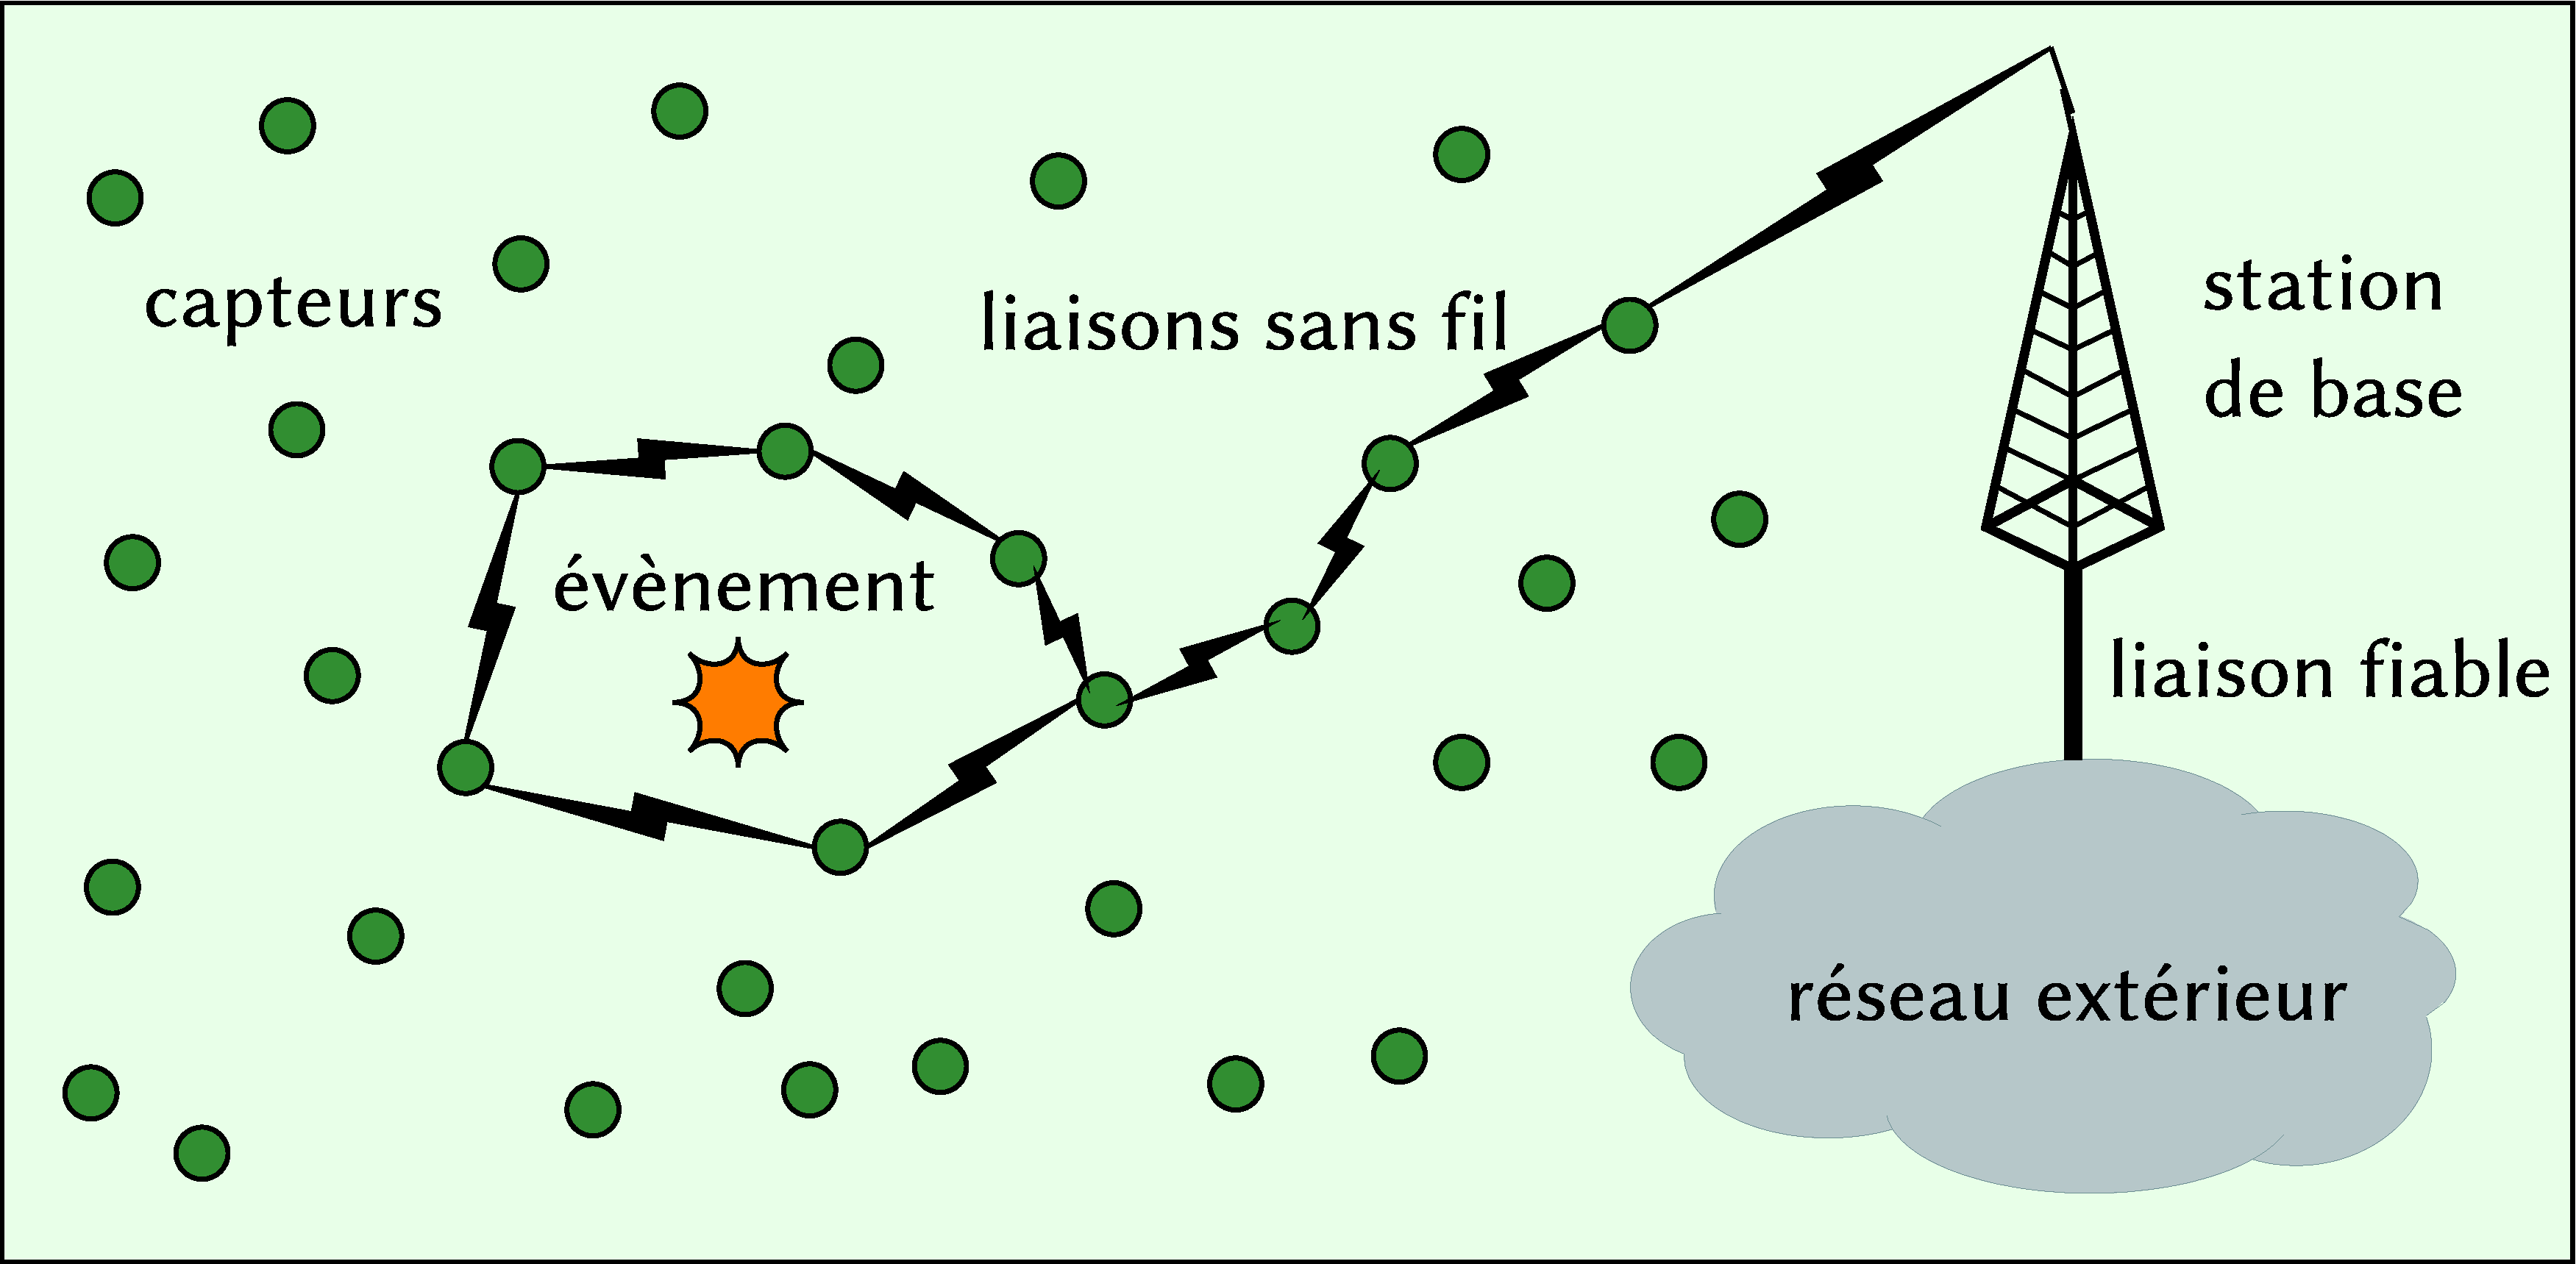
\includegraphics[height=.5\textheight]{Figs/WSN_archi.pdf}
\end{frame}
%===============================================================================
\begin{frame}{Réseaux de capteurs sans fils clusterisés}
  Quelques problématiques:
  \begin{itemize}
    \item déploiement autonome; gestion décentralisée
    \item performances; gestion de l'énergie
    \item sureté, résilience; \alert{sécurité}
  \end{itemize}
  \vfill
  Notion de \alert{clusters}:

  \smallskip
  \centering
  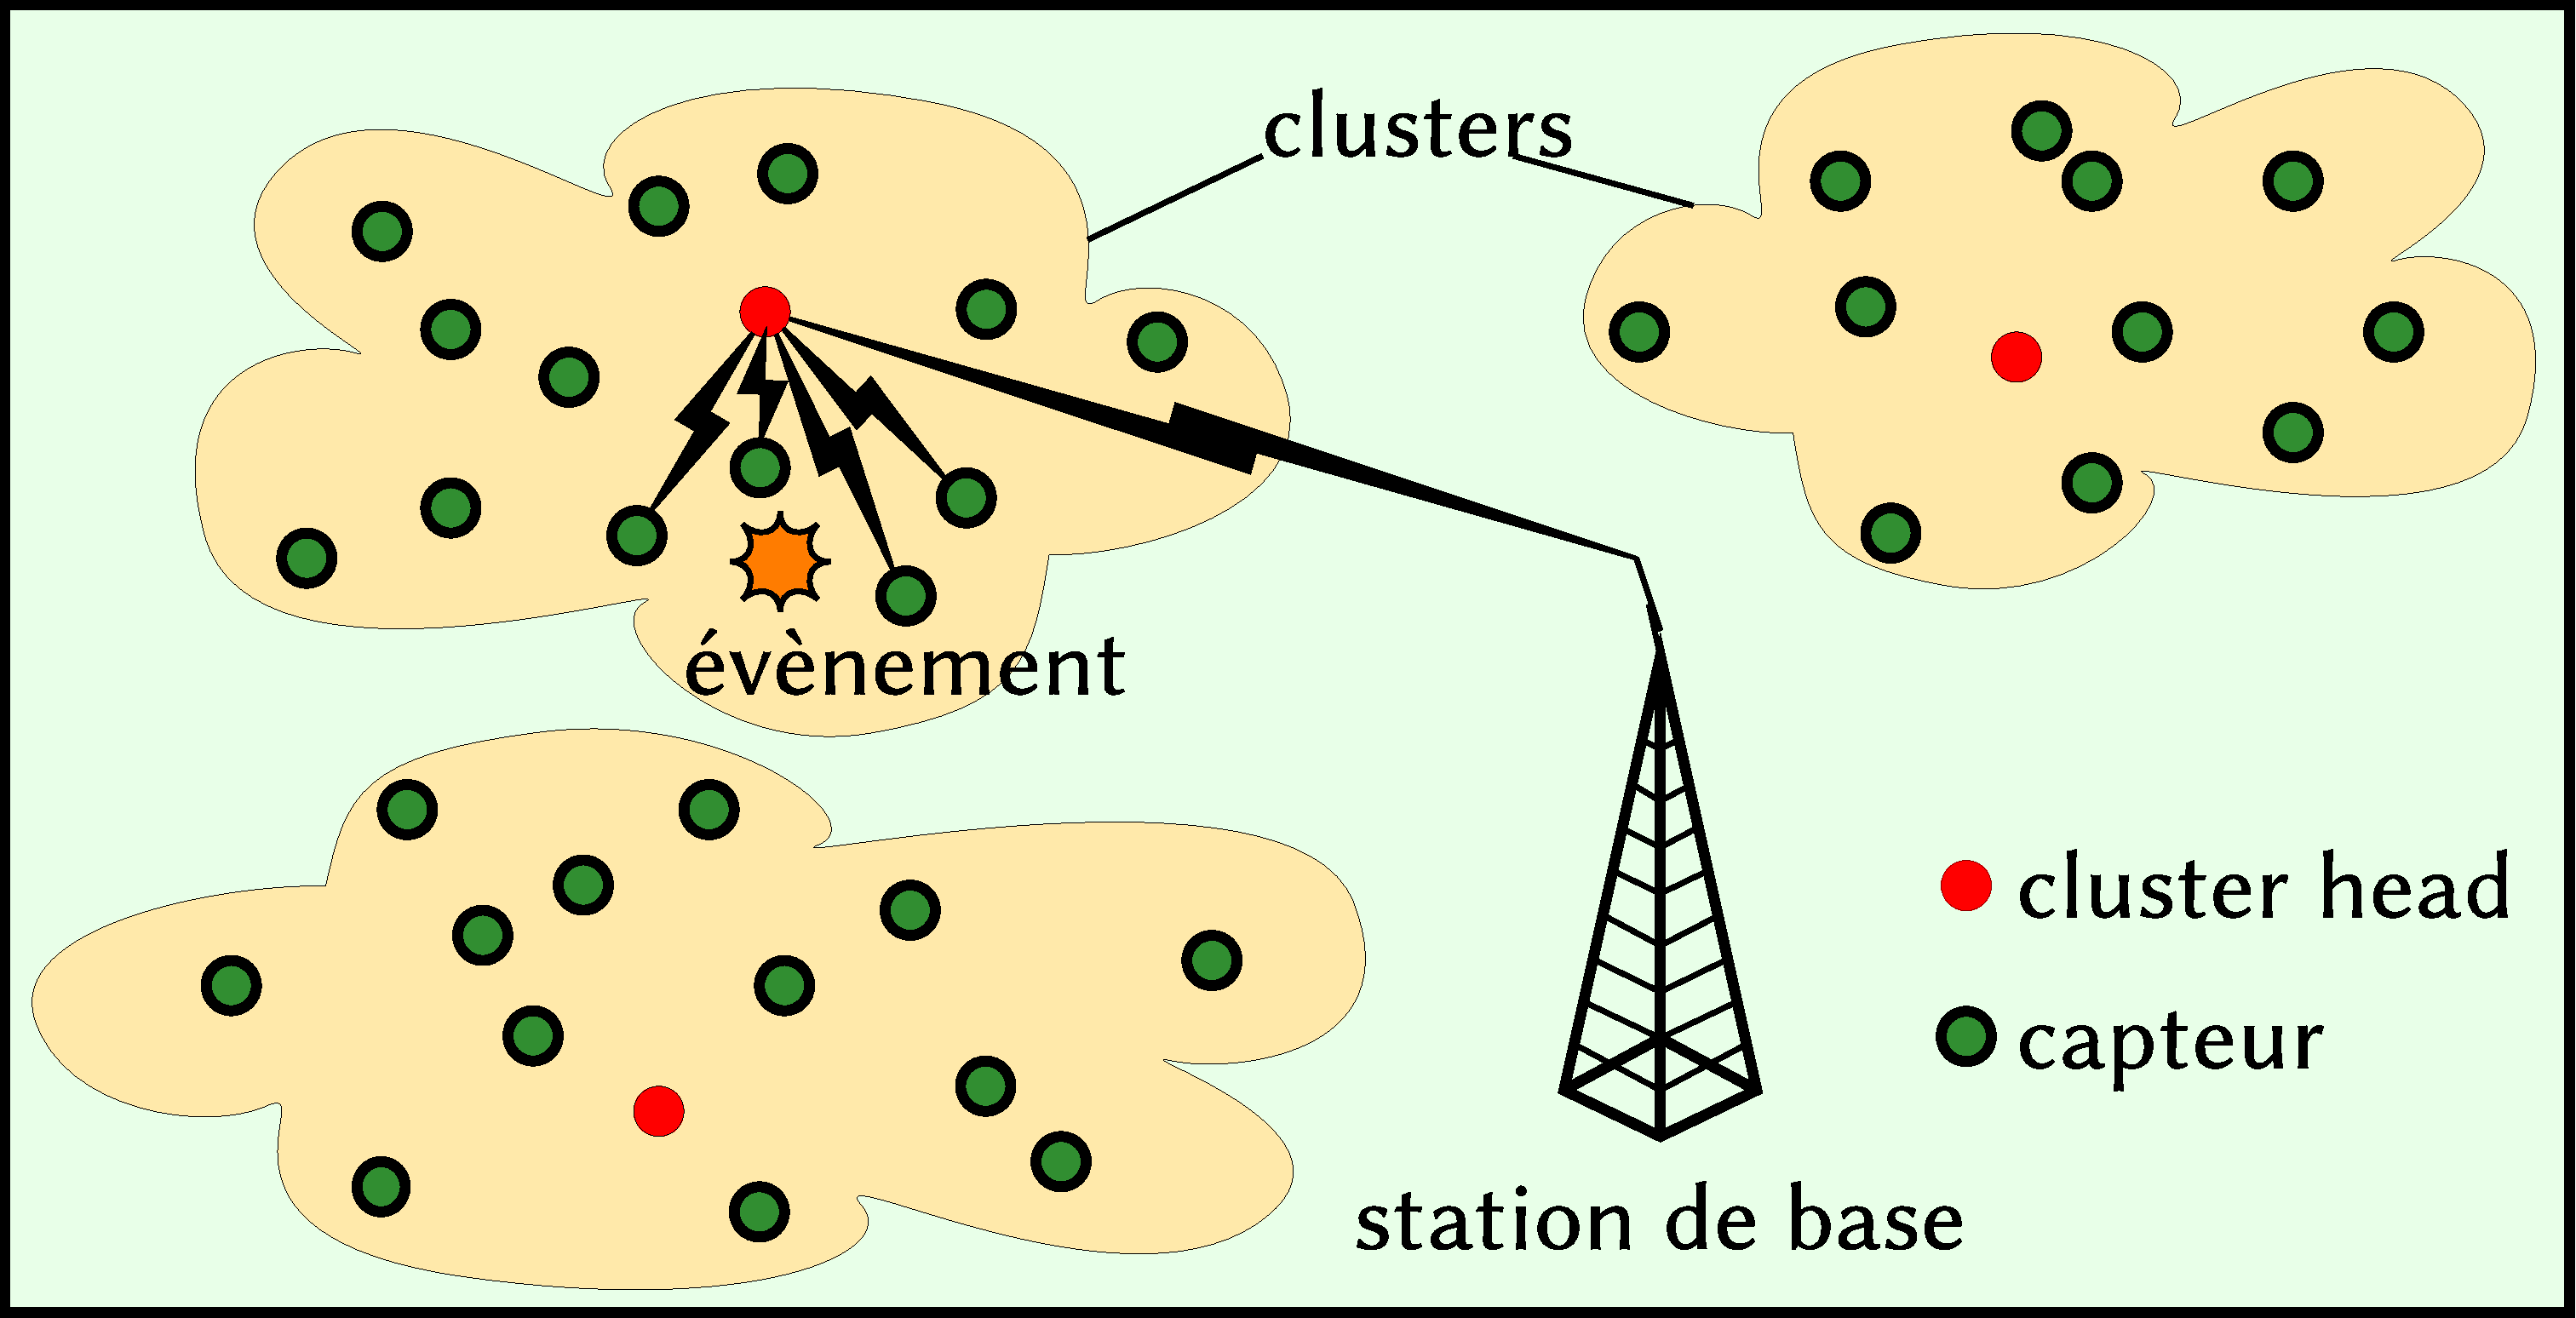
\includegraphics[height=.5\textheight]{Figs/WSN.pdf}
\end{frame}
%===============================================================================
\begin{frame}{Exemples d'applications}
  \begin{small}
    \begin{itemize}
      \item \textbf{Milieu urbain:} surveillance du trafic routier, «\,villes intelligentes\,»
      \item \textbf{Environnement:} agriculture, suivi d'animaux, mesure du taux de pollution, météo
      \item \textbf{Surveillance:} activité sismique, départs d'incendie en forêt ou sur site industriel, vidéosurveillance et détection d'intrusions (physiques)
      \item \textbf{Particuliers:} «\,Internet des objets\,», domotique
      \item \textbf{\alert{Médecine}:} surveillance d'organes vitaux ou de glycémie, détection de tumeurs
      \item \textbf{Domaine \alert{militaire}:} renseignement, détection d'agents chimiques / biologiques / radioactifs
    \end{itemize}
  \end{small}
  Fortes contraintes en sécurité
\end{frame}
%===============================================================================
\subsection[Sécurité]{Sécurité, déni de service}
%===============================================================================
\begin{frame}{Sécurité dans les réseaux de capteurs}
  Plusieurs composantes:
  \begin{small}
    \begin{itemize}
      \item Confidentialité des données
      \item Authentification, intégrité des échanges
      \item \alert{Disponibilité} des services\\
        Dans notre cas: détection des attaques par \alert{déni de service} (DoS).\\
        Plusieurs couches (pile TCP/IP) peuvent être visées:\\
        \begin{itemize}
            \footnotesize
          \item couche physique (brouillage)
          \item \alert{couche MAC} (brouillage, comportements égoïstes, privation de sommeil, \dots)
          \item \alert{routage} (trous noirs, trous de vers, attaques sur le protocole de routage, \dots)
          \item couche transport (tempêtes SYN/ACK sur TCP/UDP, \dots)
          \item applications
        \end{itemize}
    \end{itemize}
  \end{small}
\end{frame}
%===============================================================================
\begin{frame}{Attaques étudiées}
  Objectif: détecter des \alert{capteurs compromis} qui tenteraient de nuire au réseau depuis l'intérieur.
  \begin{itemize}
    \item Les capteurs compromis font partie du réseau (même matériel)
    \item Ils effectuent des attaques sur les couches MAC (contrôle d'accès au médium) ou de routage IP, par exemple:
      \begin{itemize}
        \item non retransmission de paquets
        \item brouillage, saturation du canal, comportement égoïste
      \end{itemize}
  \end{itemize}
  \medskip
  Contrainte: \alert{limiter} et \alert{répartir} la consommation en énergie
\end{frame}
%===============================================================================
\section[Mécanismes]{Sélection des capteurs de surveillance}
%===============================================================================
\begin{frame}{Détection des attaques}
  \small
  Mécanisme de détection des comportements suspects
  \begin{itemize}
    \item Sous-ensemble de capteurs (\alert{\cnsns}) chargés d'établir une surveillance du trafic
    \item Application d'un ensemble de \alert{règles} sur le trafic observé
    \item Si détection d'un comportement suspect, remontée d'une alarme au \ch
      \smallskip
      \begin{center}
        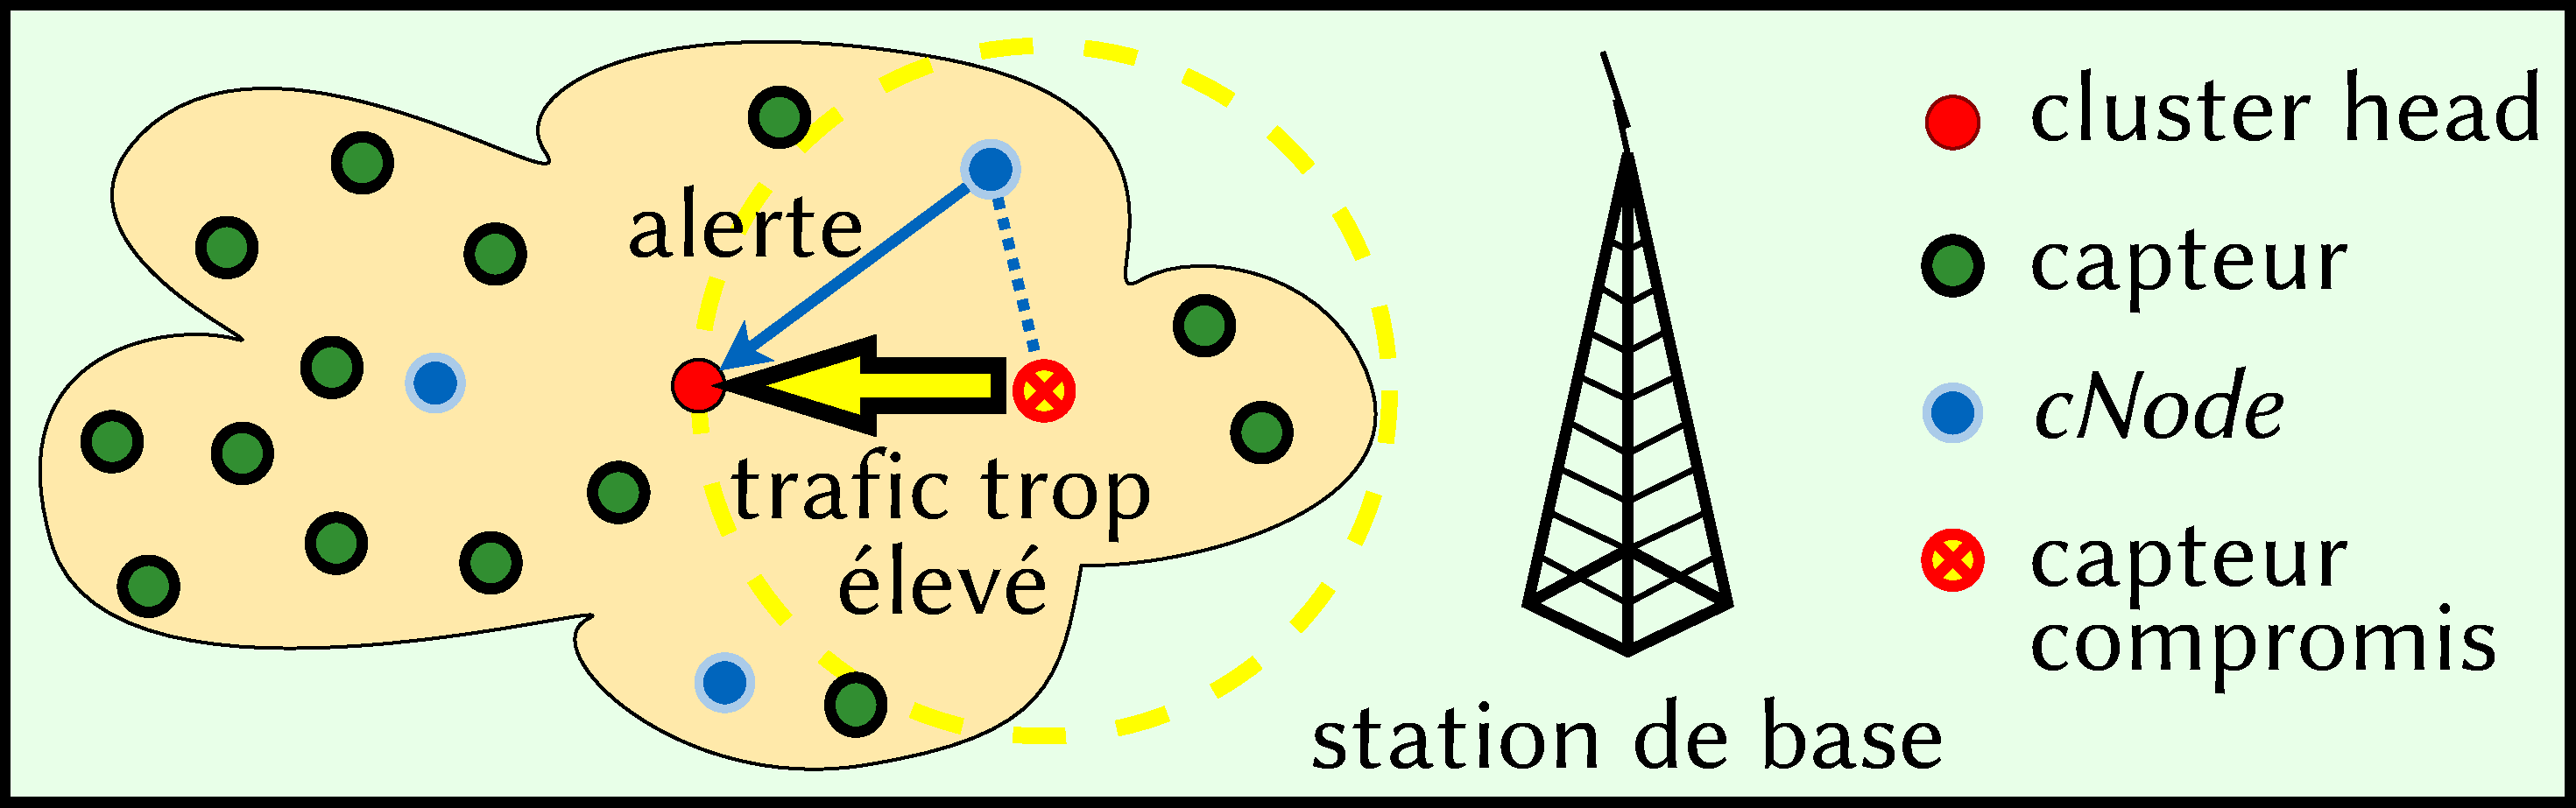
\includegraphics[height=.3\textheight]{Figs/WSN_detection.pdf}
      \end{center}
    \item \alert{Renouvellement périodique des \cns}
  \end{itemize}
  \begin{block}{Problème posé:}
    Pour chaque période, comment sélectionner les \cns?
  \end{block}
\end{frame}
%===============================================================================
\begin{frame}{Trois méthodes de renouvellement}
  \begin{enumerate}
    \item Sélection aléatoire
    \item Sélection selon l'énergie résiduelle
    \item Élection démocratique
  \end{enumerate}
  Résultats numériques: simulations
\end{frame}
%===============================================================================
\subsection{Sélection aléatoire}
%===============================================================================
\begin{frame}{Sélection aléatoire des \cns}
  \begin{itemize}
    \item Méthode simple
    \item Dans la littérature: rien sur le renouvellement de la sélection des \cns au cours du temps [\textsc{Lai} et \textsc{Chen}, 2008]
    \item Ce qui importe: assurer ce renouvellement
  \end{itemize}
  \begin{block}{Principe}
    Déterminer la liste des \cns de façon aléatoire, à l'aide d'un générateur de nombres (pseudo-)aléatoires
  \end{block}
\end{frame}
%===============================================================================
\begin{frame}{Sélection aléatoire des \cns\ --- implémentation}
  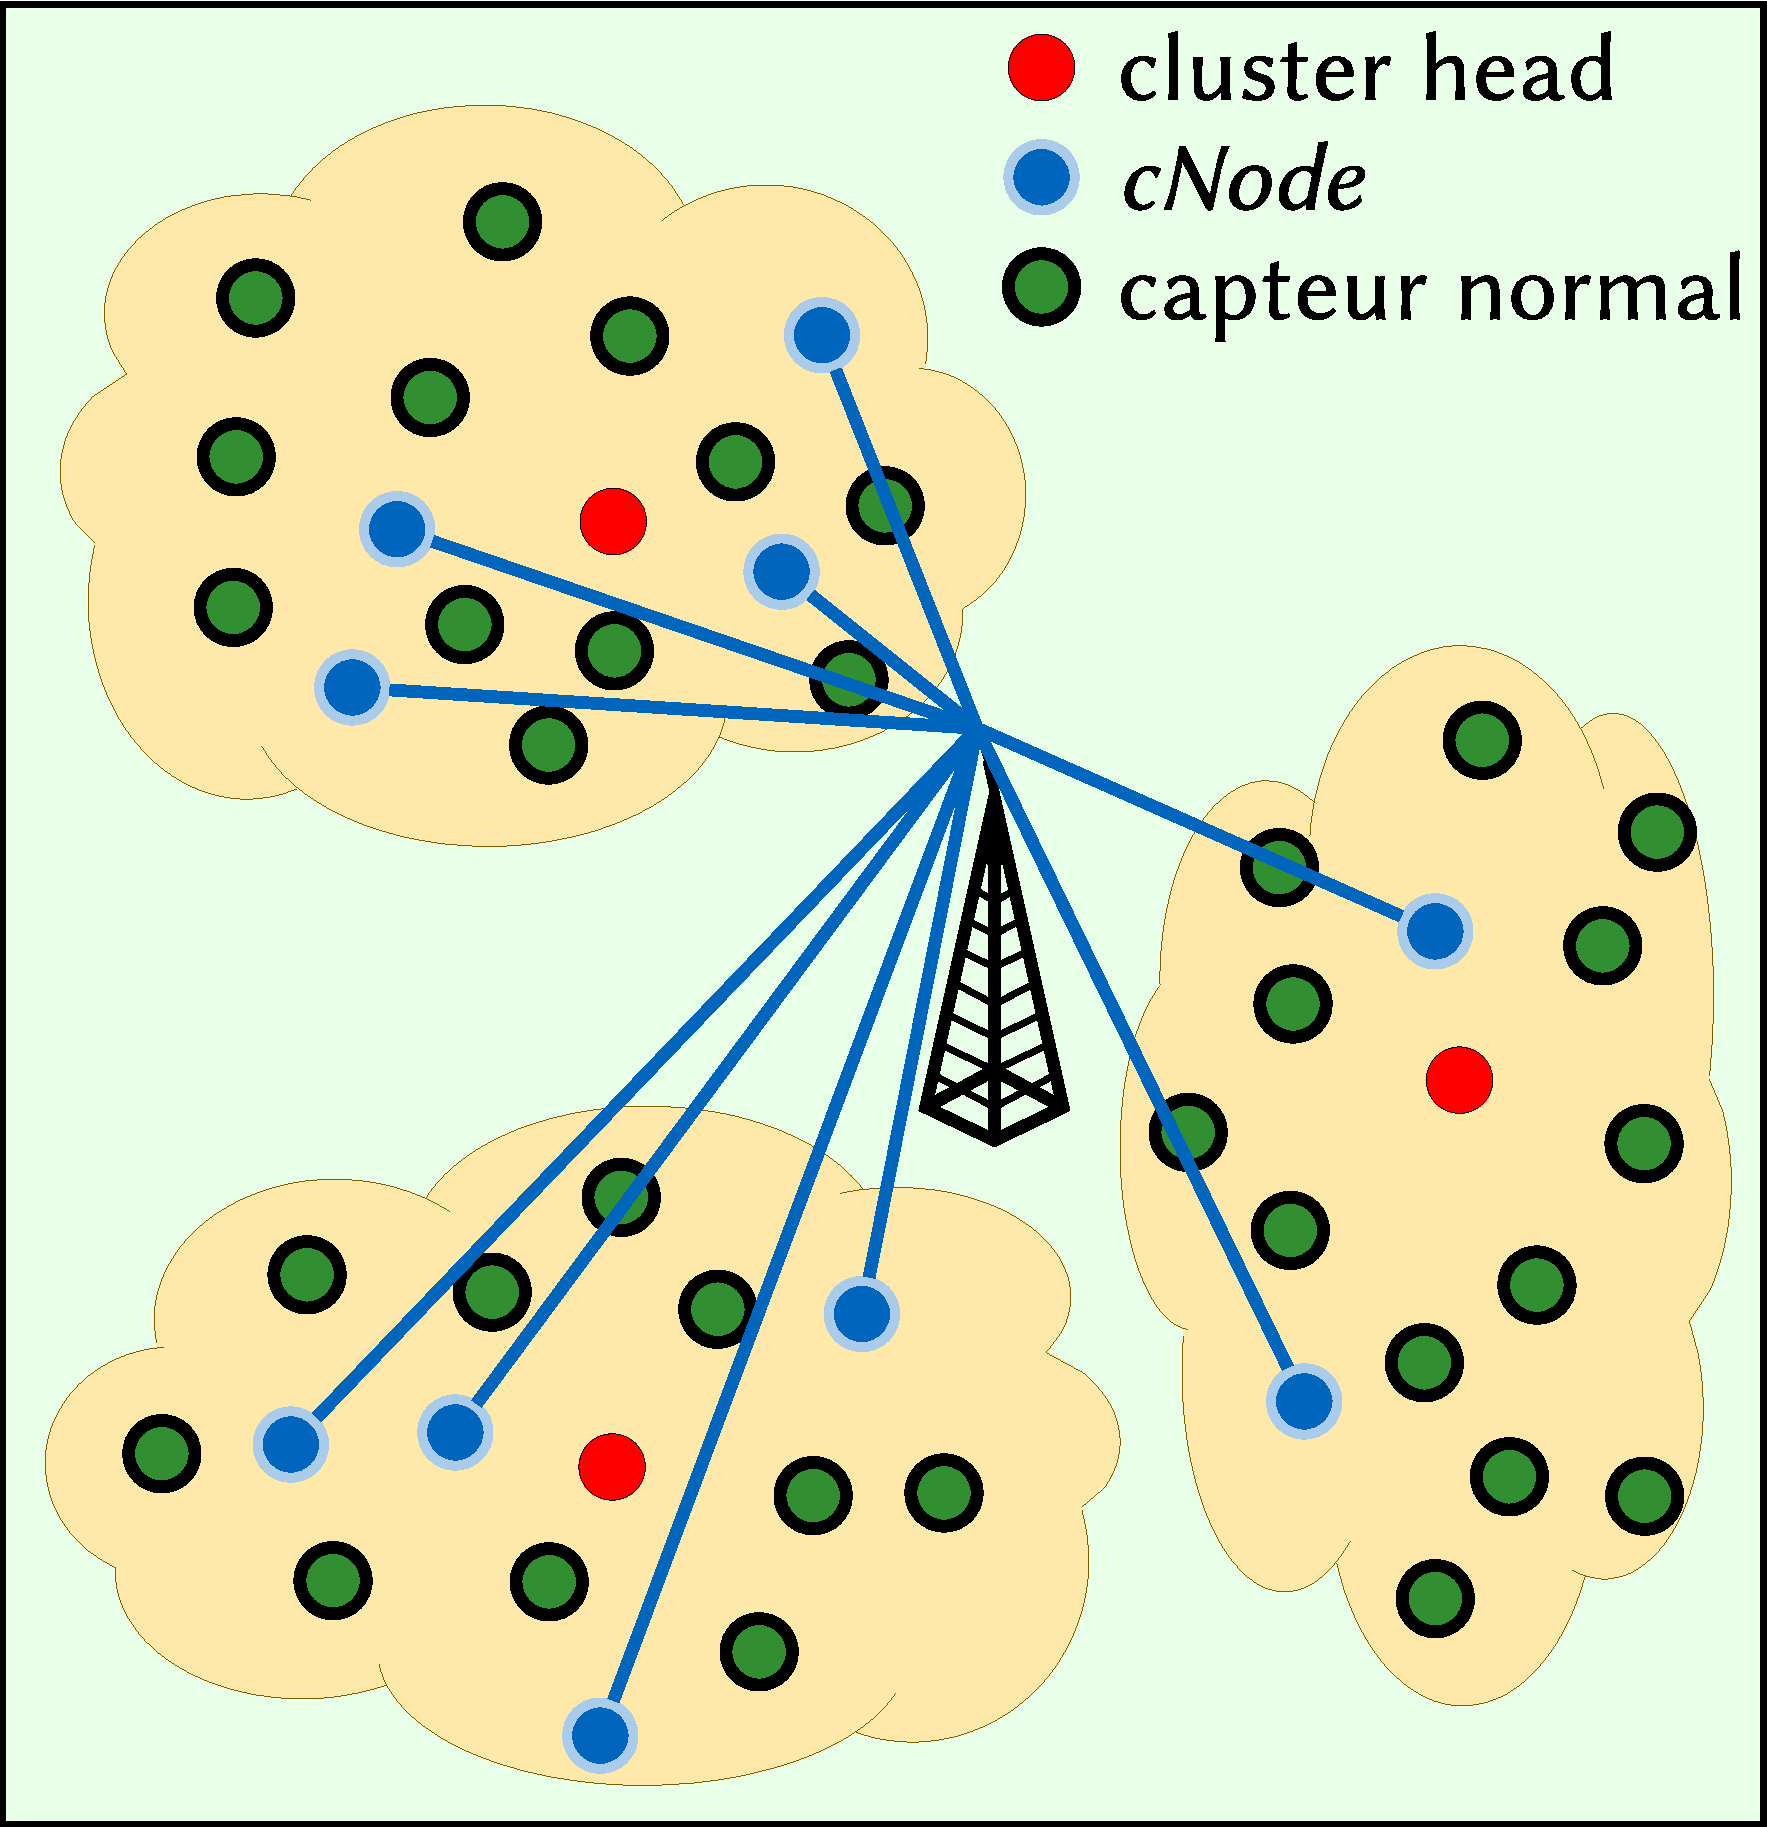
\includegraphics[height=.4\textheight]{Figs/elec_bs.pdf}\hfill
  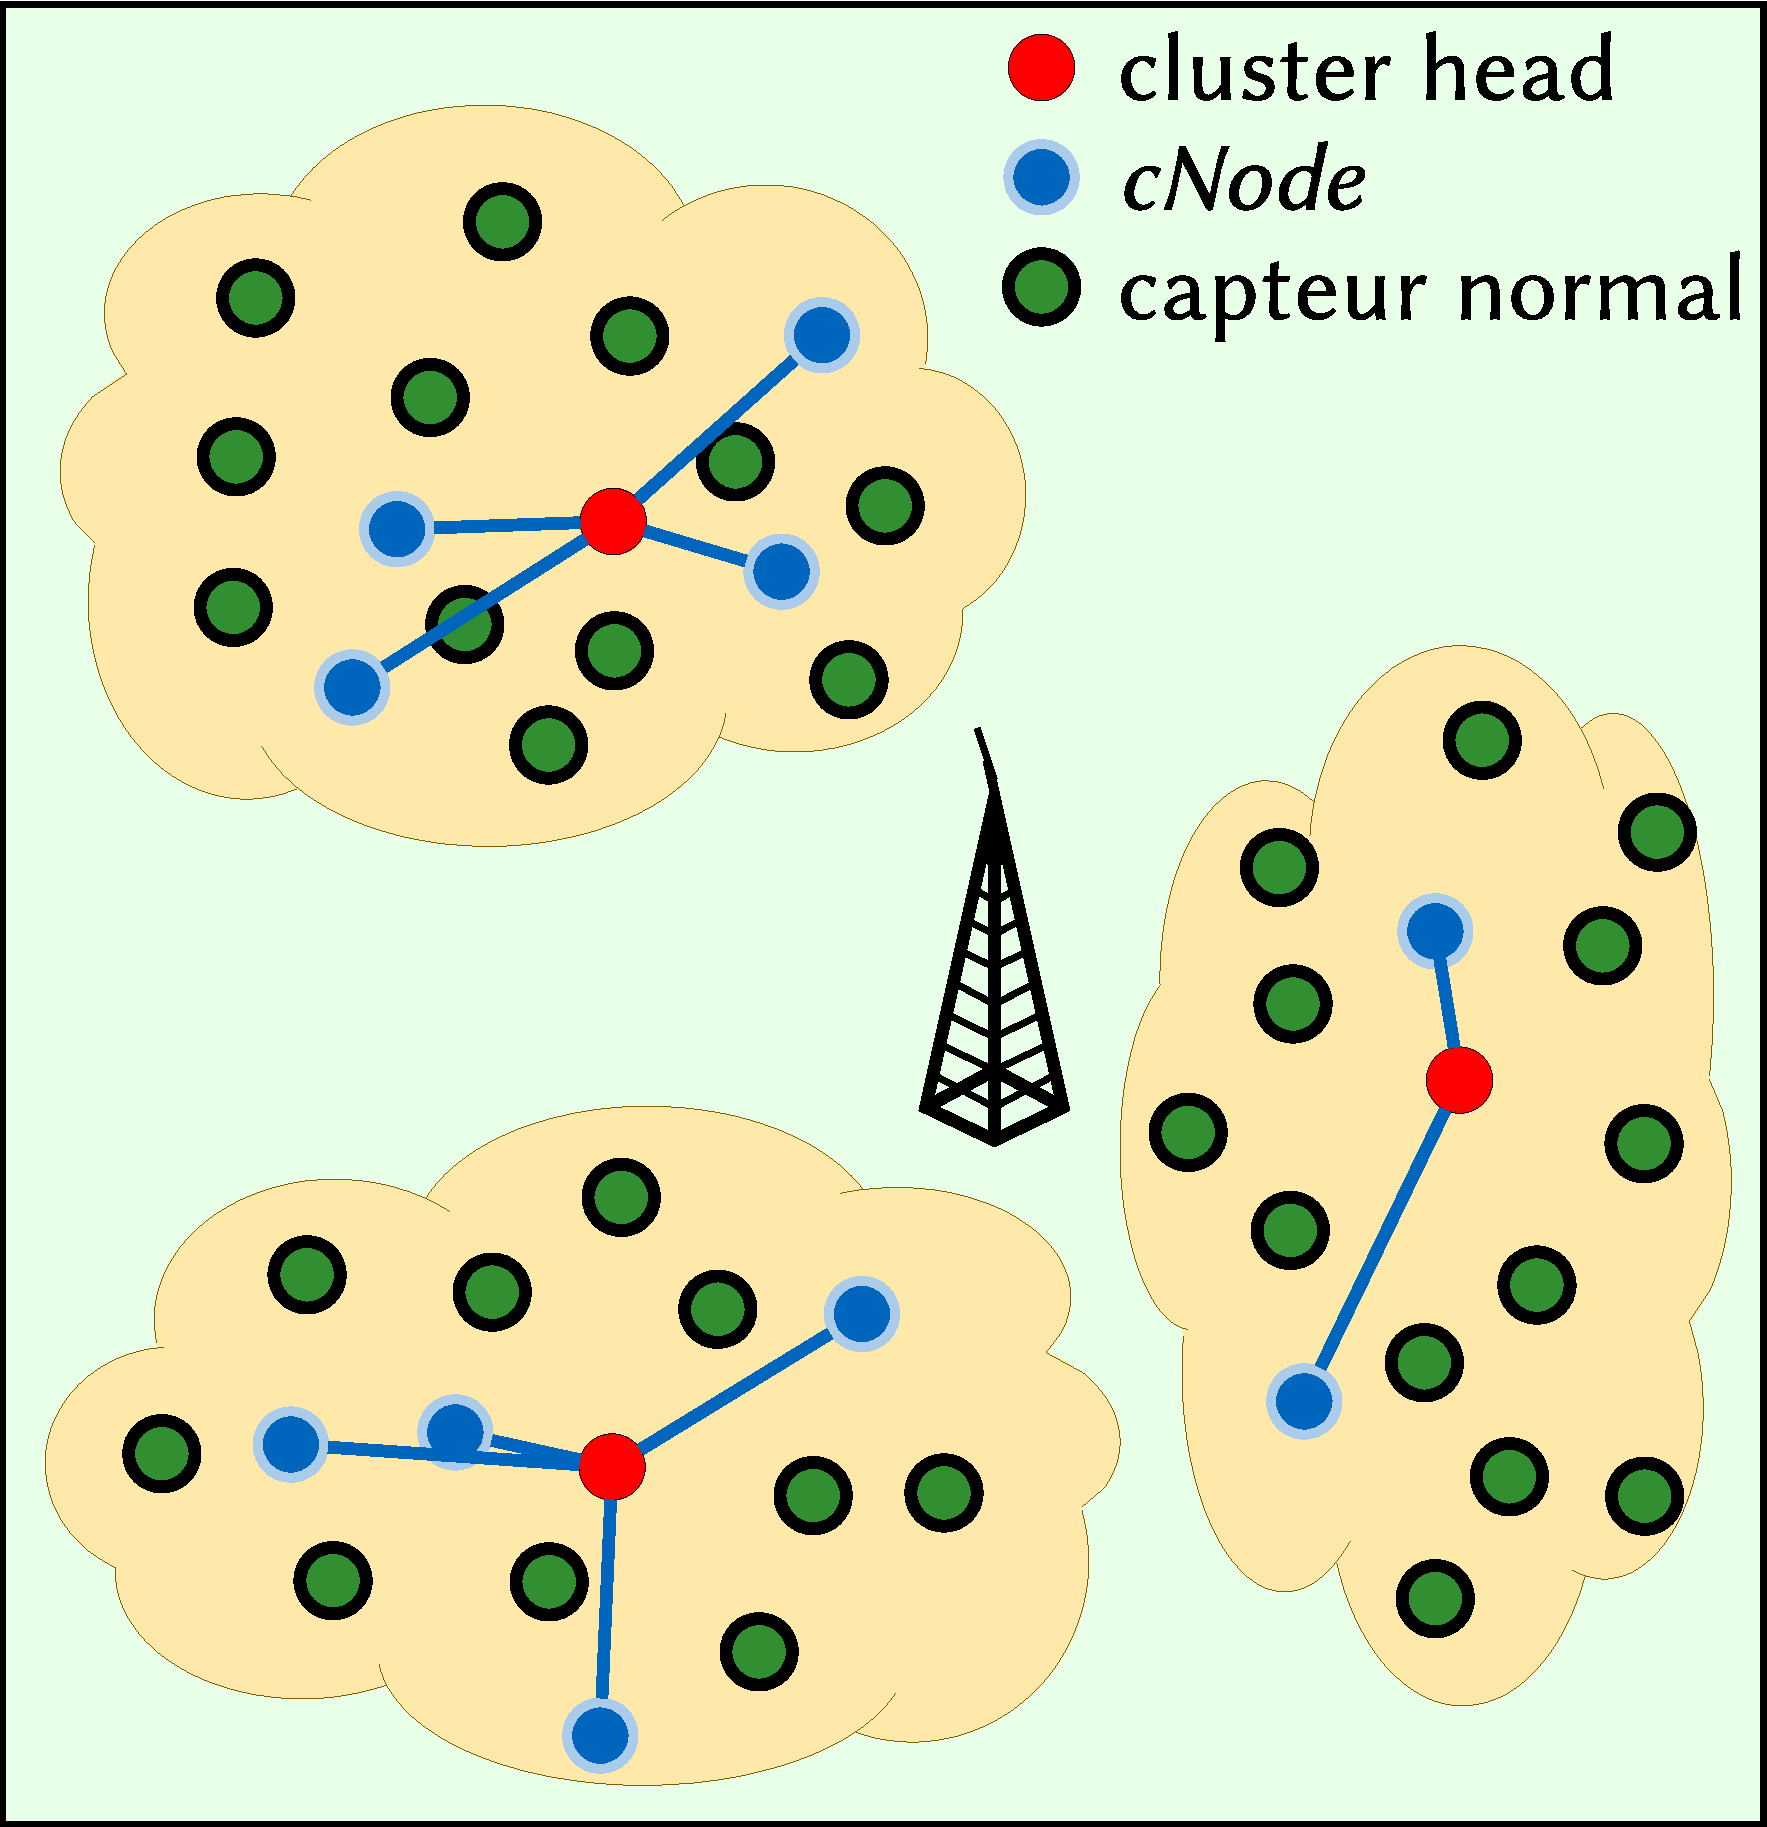
\includegraphics[height=.4\textheight]{Figs/elec_ch.pdf}\hfill
  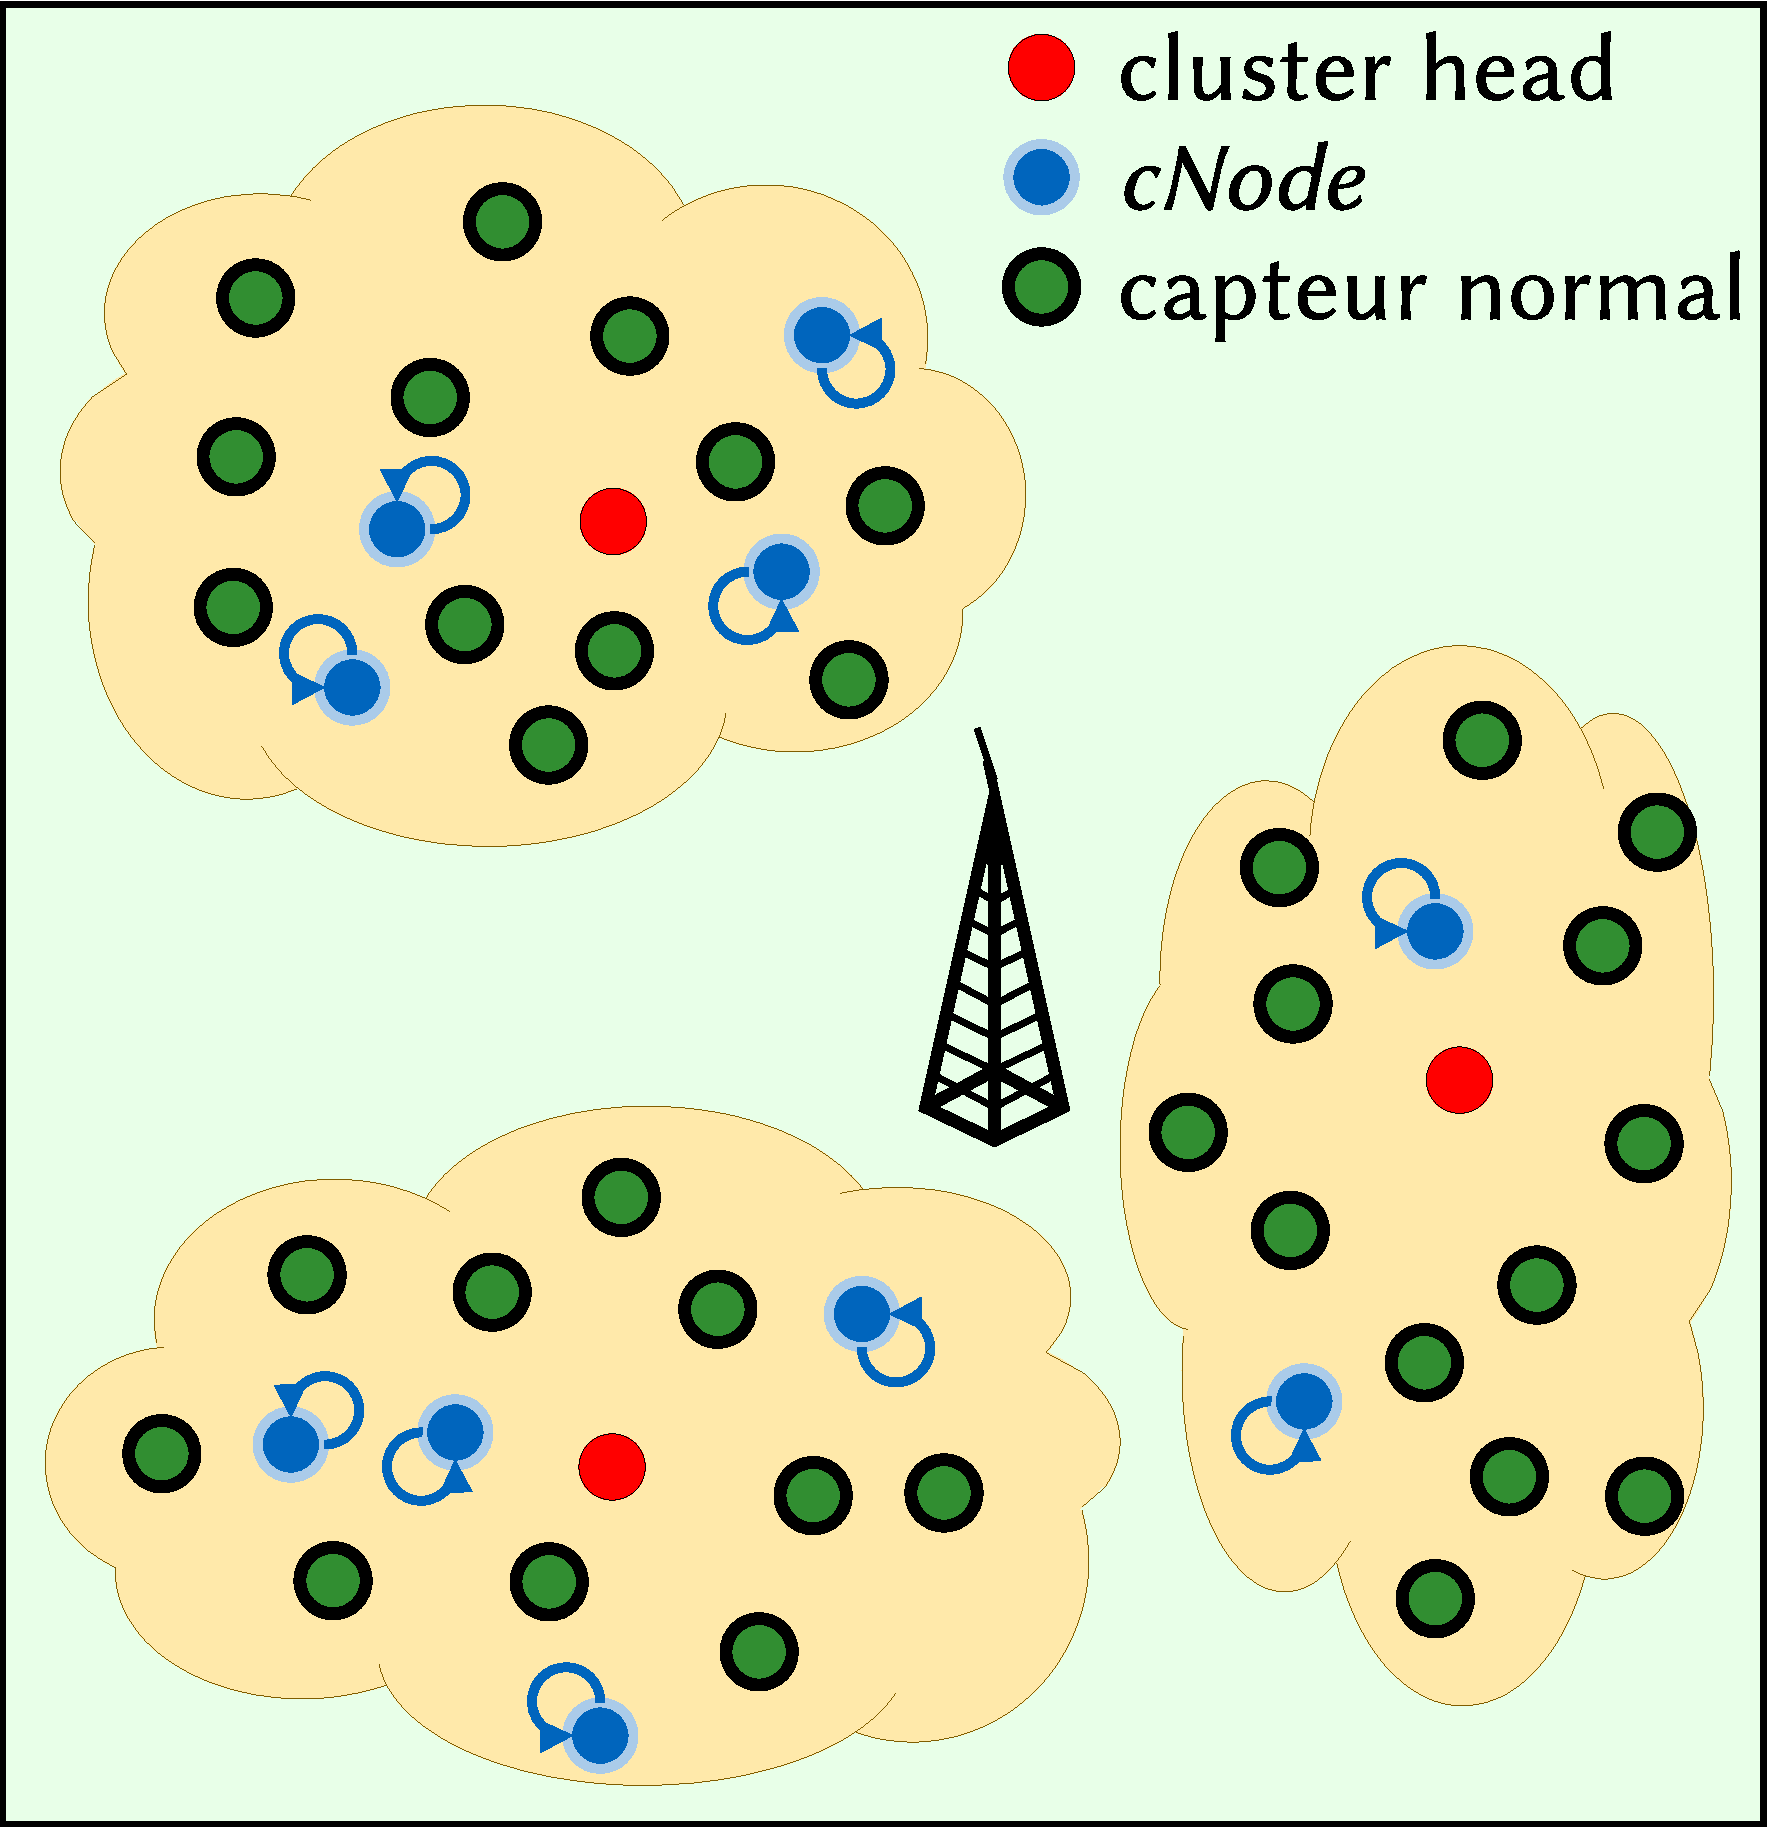
\includegraphics[height=.4\textheight]{Figs/elec_self.pdf}

  \bigskip
  \scriptsize
  \begin{tabu}{X[1,c,m] X[2,l,m] X[2.3,j,m]}
    \textsc{Méthode} & \centering \textsc{Avantages} & \centering \textsc{Inconvénients} \tabularnewline
    \midrule
    Sélection par la station de base & %
    \textbullet\;Aucun calcul des capteurs\newline%
    \textbullet\;Distribution spatiale idéale%
    & %
    \textbullet\;Si le \CH est compromis, il déclare un cluster vide\newline%
    \textbullet\;Perte de l'aspect décentralisé de l'algorithme\tabularnewline
    \midrule
    Sélection par les \chs & %
    \textbullet\;Seuls les \CH calculent les nombres aléatoires%
    & %
    \textbullet\;Si le \CH est compromis, il ne désigne aucun \cn \tabularnewline
    \midrule
    Auto-sélection & %
    \textbullet\;Très simple\newline%
    \textbullet\;Peu de données de contrôle%
    & %
    \textbullet\;Chaque capteur calcule un nombre aléatoire\newline%
    \textbullet\;Ignore la topologie du réseau\tabularnewline
  \end{tabu}
\end{frame}
%===============================================================================
\subsection[Énergie résiduelle]{Selon l'énergie résiduelle}
%===============================================================================
\begin{frame}{Sélection des \cns selon l'énergie résiduelle}
  \begin{block}{Principe}
    Les capteurs dont le niveau de charge de batterie est le plus élevé sont sélectionnés en tant que \cns
  \end{block}
  Algorithme déterministe

  \begin{minipage}{.6\textwidth}
    \begin{colorblock}
      \begin{block}{Problèmes:}
        \begin{enumerate}
          \item Comment empêcher les capteurs compromis d'accaparer le rôle de \cn?
          \item Comment être sûr de couvrir tout le cluster?
        \end{enumerate}
      \end{block}
    \end{colorblock}
  \end{minipage}\hfill
  \begin{minipage}{.39\textwidth}
    \raggedleft
    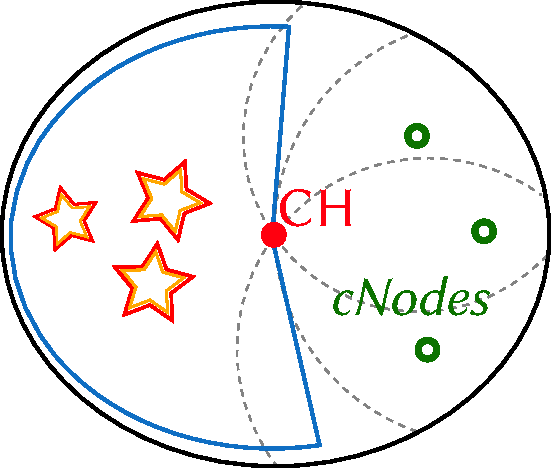
\includegraphics[height=.35\textheight]{Figs/cover.pdf}
  \end{minipage}
\end{frame}
%===============================================================================
\begin{frame}{Sélection selon l'énergie résiduelle --- solutions}
  \begin{block}{Solutions:}
    \begin{enumerate}
      \item Nouveau type de capteurs: les \vns
      \item Chaque capteur surveillé par au moins deux \cns
    \end{enumerate}
  \end{block}
  Les \vns surveillent la consommation énergétique des \cns à l'aide d'un modèle mathématique
  \vfill
  \centering
  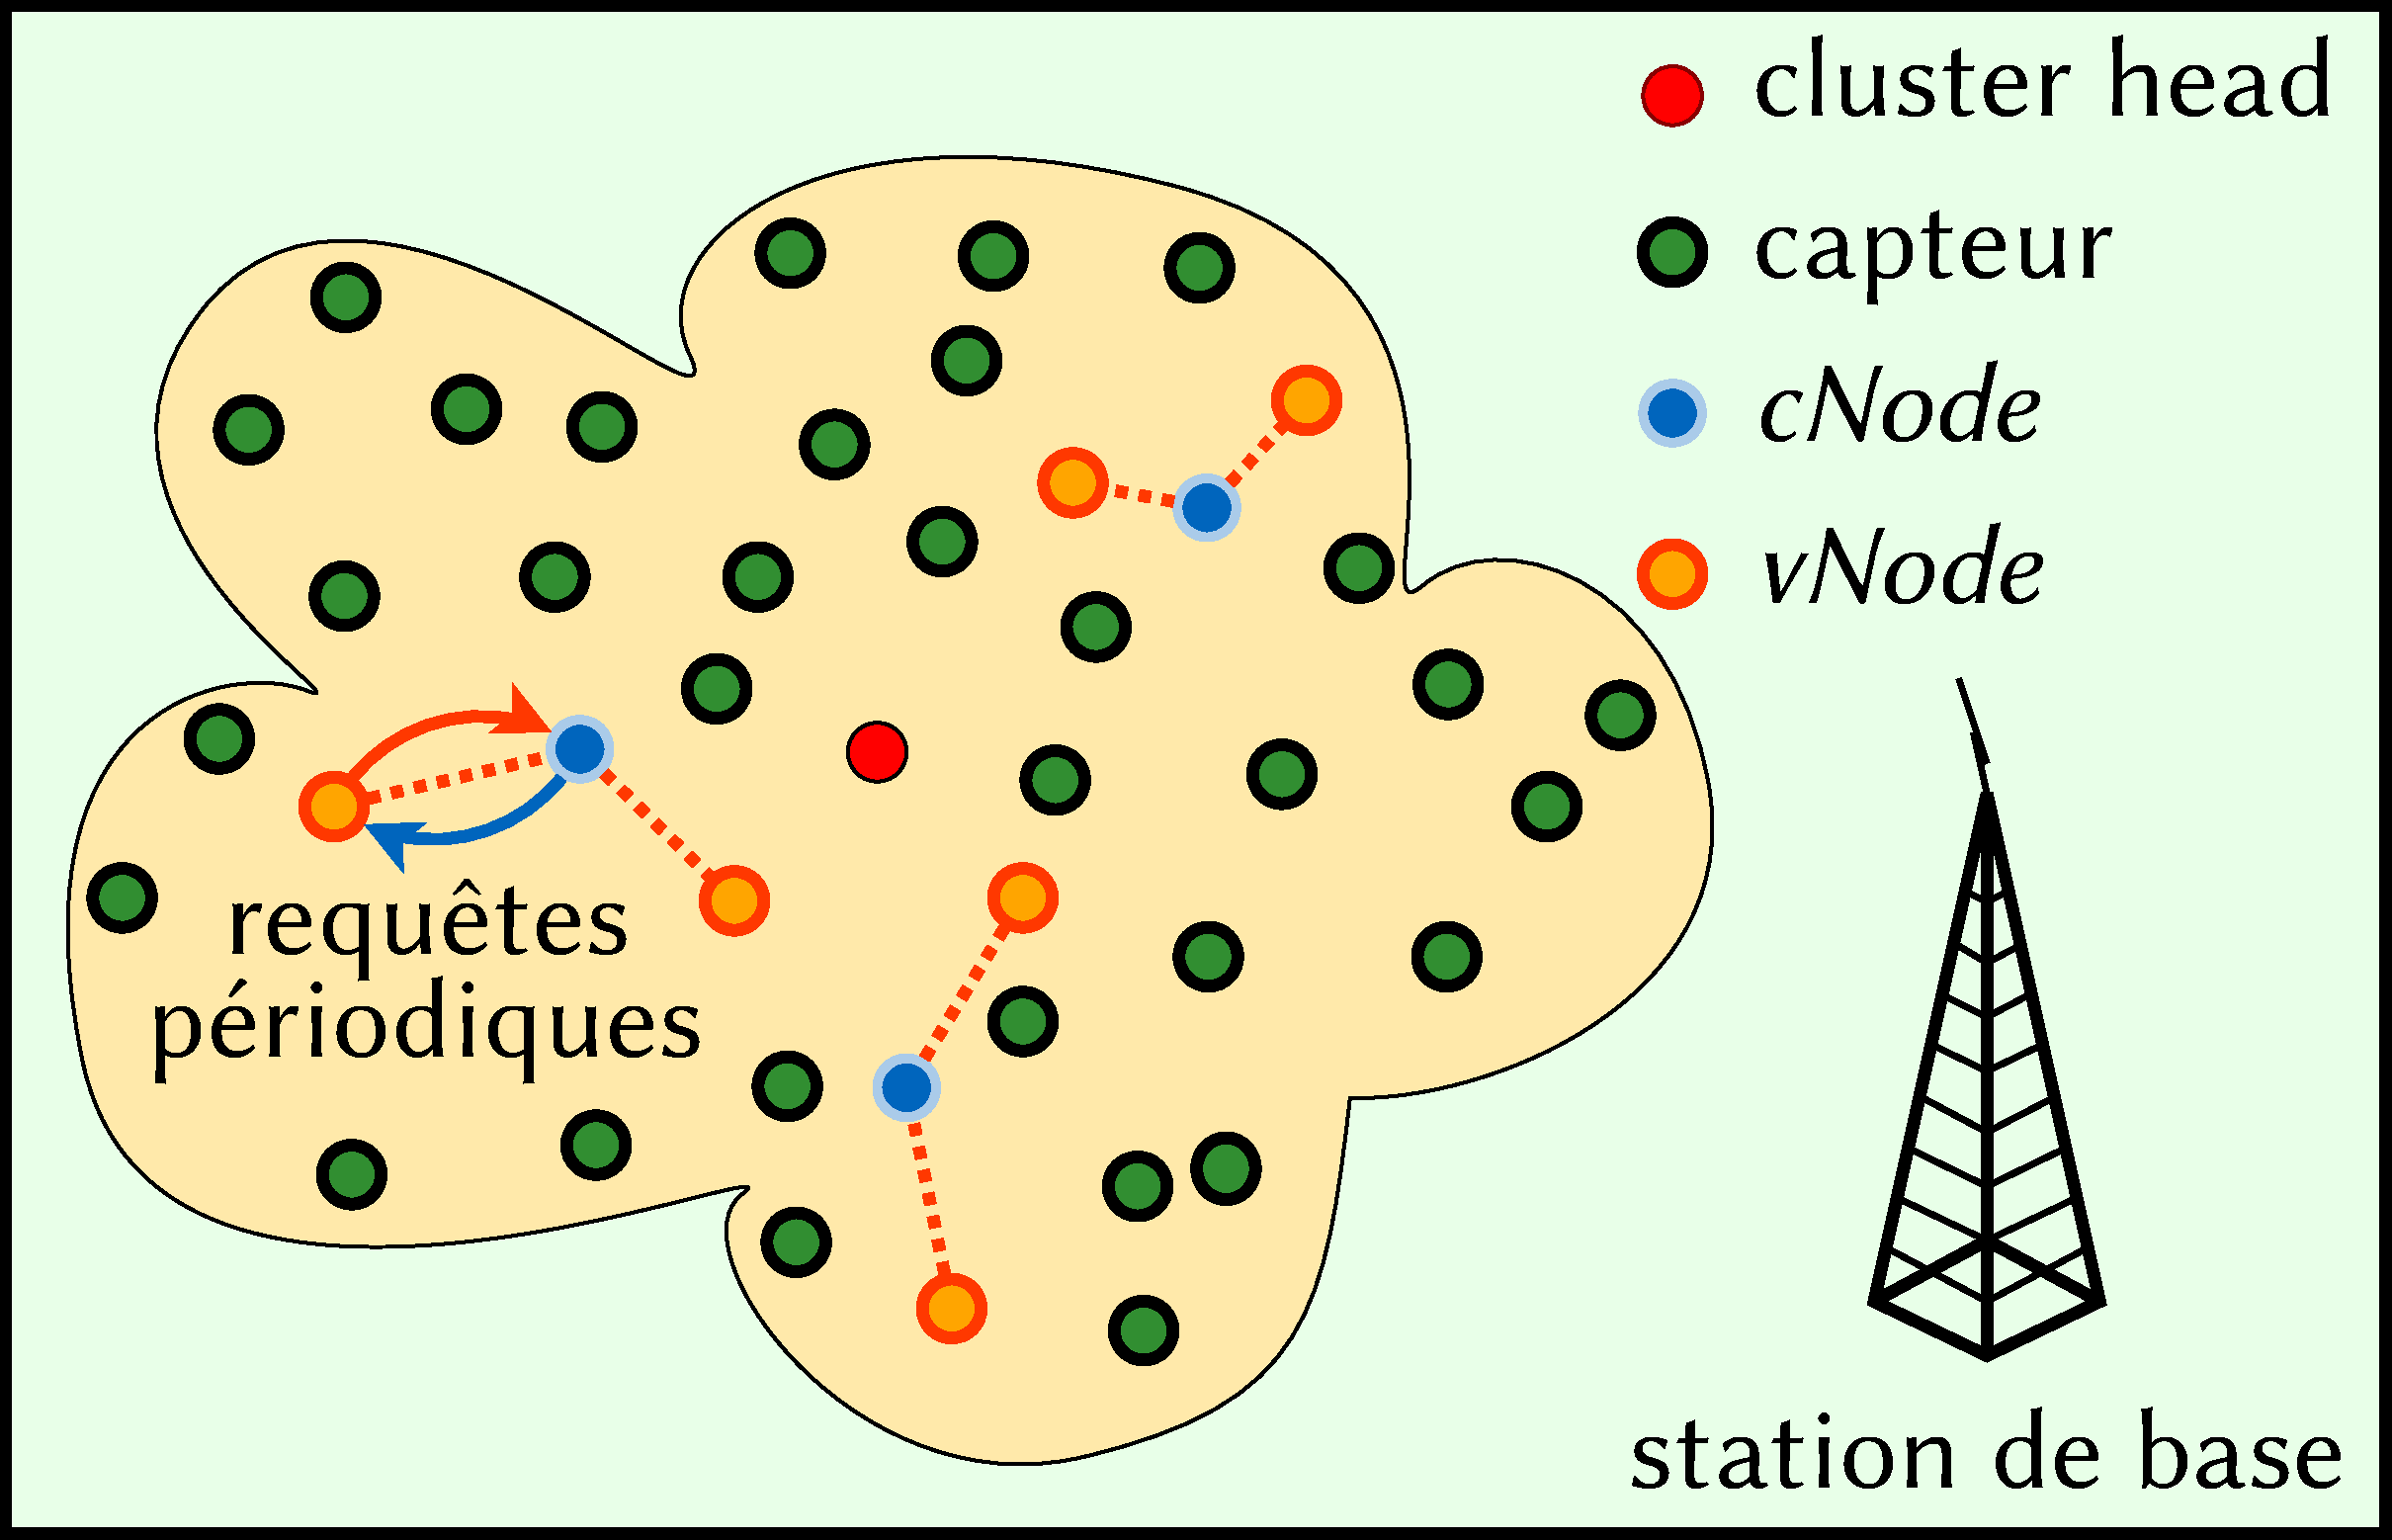
\includegraphics[width=.6\textwidth]{Figs/WSN_vNodes.pdf}
\end{frame}
%===============================================================================
\subsection{Élection démocratique}
%===============================================================================
\begin{frame}{Élection démocratique des \cns}
  \begin{block}{Principe}
    Les observations réalisées par les capteurs sur leurs voisins sont utilisées pour élire (auprès du \ch) les nouveaux \cns
  \end{block}
  Deux étapes:
  \begin{enumerate}
    \item Une phase initiale où tous les capteurs observent leurs voisins
    \item Puis fonctionnement standard: les \cns envoient leurs observations (leurs «\,votes\,») au \ch
  \end{enumerate}
  \bigskip
  Le vote peut prendre en compte plusieurs critères:
  \begin{footnotesize}
    \begin{eqnarray*}
      \textit{note}_k[i\:\!] & = & (\alpha \times \textit{énergie\_résiduelle}_k[i\:\!]) + (\beta \times \textit{réputation}_k[i\:\!])\\
                             & + & (\gamma \times \textit{index\_connectivité}_k[i\:\!]) + (\delta \times \textit{puissance du signal}_k[i\:\!])\\
                             & + & (\zeta  \times \textit{durée\_depuis\_dernière\_sélection}_k[i\:\!])
    \end{eqnarray*}
  \end{footnotesize}
\end{frame}
%===============================================================================
\subsection{Résultats}
%===============================================================================
\begin{frame}{Simulations --- système simulé}
  Logiciel utilisé: ns (network simulator)

  {\small Grille de 100 capteurs}

  \bigskip
  \begin{minipage}{.5\textwidth}
    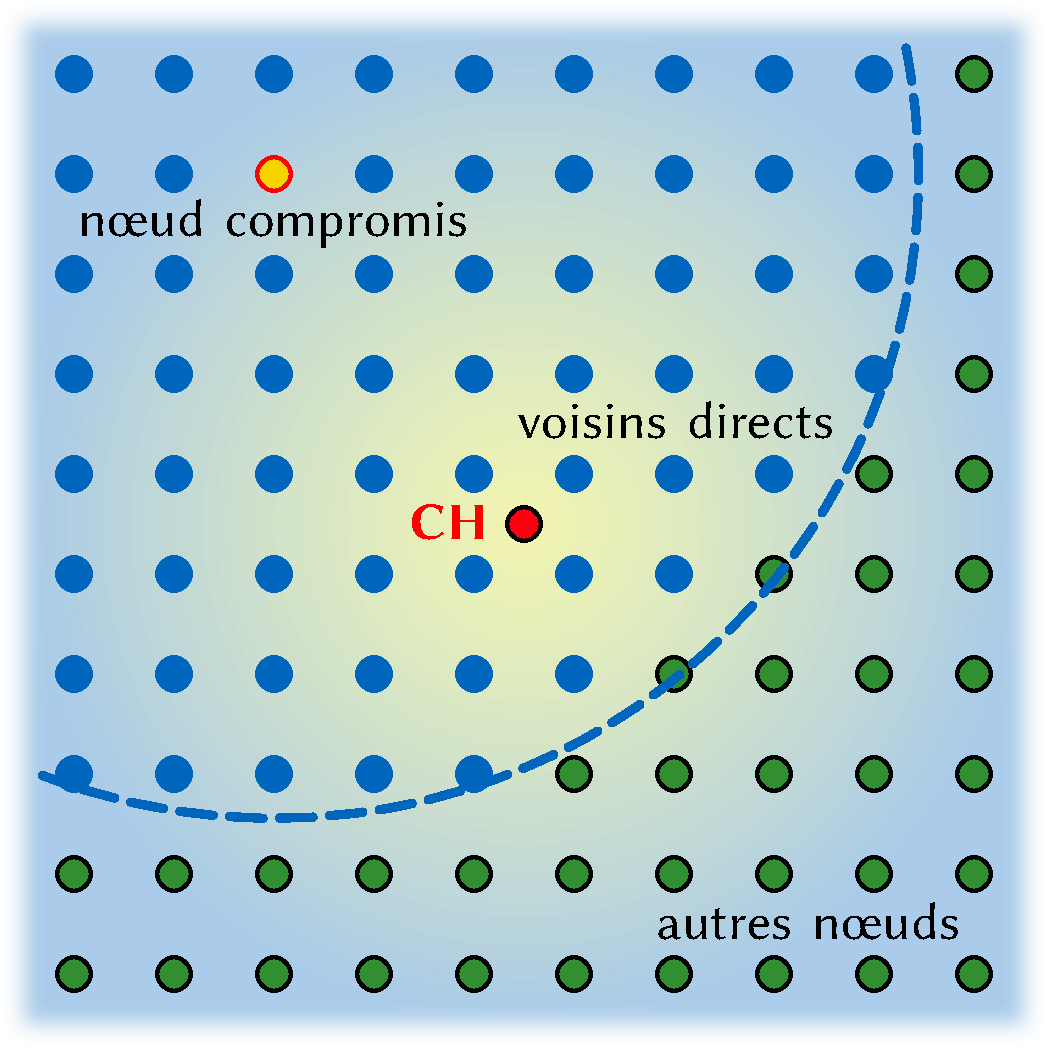
\includegraphics[height=.7\textheight]{Figs/WSN_neighbors.pdf}
  \end{minipage}\hfill
  \begin{minipage}{.42\textwidth}
    5 cas pour le renouvellement des \cns:
    \begin{itemize}
      \item sans renouvellement
      \item aléatoire (10 \cns)
      \item énergie résiduelle (10~\cns)
      \item élec.\ dém. (10 \cns)
      \item élec.\ dém. (7 \cns)
    \end{itemize}
  \end{minipage}
\end{frame}
%===============================================================================
\begin{frame}{Simulations --- énergie consommée}
  \begin{minipage}{.65\textwidth}
    \includegraphics[height=.48\textheight]{Figs/plot_sd_consumptionXtime.pdf}
  \end{minipage}
  \begin{minipage}[c][.48\textheight][t]{.34\textwidth}
    \raggedright\medskip
    Énergie consommée (moyenne)
  \end{minipage}
  \begin{minipage}[c][.48\textheight][b]{.34\textwidth}
    \raggedright
    Énergie consommée (écart-type)
    \bigskip
  \end{minipage}
  \begin{minipage}{.65\textwidth}
    \raggedleft
    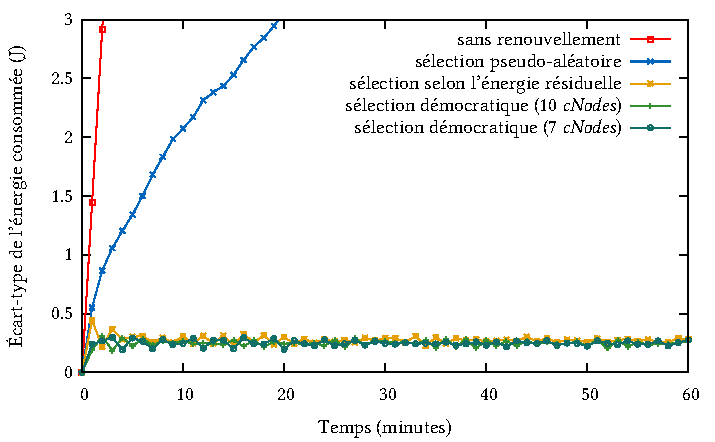
\includegraphics[height=.48\textheight]{Figs/plot_sd_stddevXtime.pdf}
  \end{minipage}
\end{frame}
%===============================================================================
\begin{frame}{Simulations --- nombre de capteurs «\,en vie\,»}
  \begin{minipage}[c][.48\textheight][t]{.34\textwidth}
    \raggedright\medskip
    Nombre de capteurs en fonctionnement au cours du temps (énergie initiale: 10~J)
  \end{minipage}
  \begin{minipage}{.65\textwidth}
    \raggedleft
    \includegraphics[height=.48\textheight]{Figs/plot_sd_nbnodesXtime_10J.pdf}
  \end{minipage}
  \begin{minipage}{.65\textwidth}
    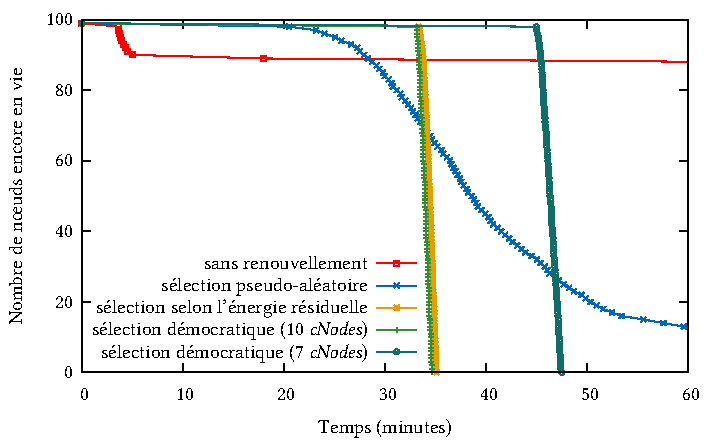
\includegraphics[height=.48\textheight]{Figs/plot_sd_nbnodesXtime_20J.pdf}
  \end{minipage}
  \begin{minipage}[c][.48\textheight][b]{.34\textwidth}
    \raggedright
    Nombre de capteurs en fonctionnement au cours du temps (énergie initiale: 20~J)
    \bigskip
  \end{minipage}
\end{frame}
%===============================================================================
\begin{frame}{Simulations --- détection au cours du temps}
  \begin{minipage}{.65\textwidth}
    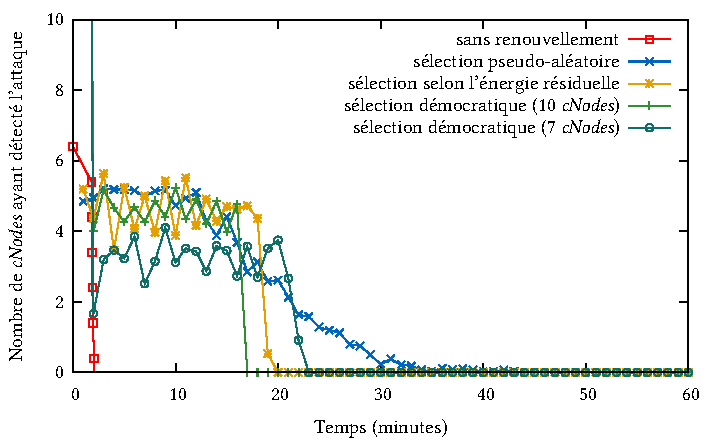
\includegraphics[height=.48\textheight]{Figs/plot_sd_detectionXtime-minute_10J.pdf}
  \end{minipage}
  \begin{minipage}[c][.48\textheight][t]{.34\textwidth}
    \raggedright\medskip
    Nombre de \cns détectant l'attaque au cours du temps (énergie initiale: 10~J)
  \end{minipage}
  \begin{minipage}[c][.48\textheight][b]{.34\textwidth}
    \raggedright
    Nombre de \cns détectant l'attaque au cours du temps (énergie initiale: 20~J)
    \bigskip
  \end{minipage}
  \begin{minipage}{.65\textwidth}
    \raggedleft
    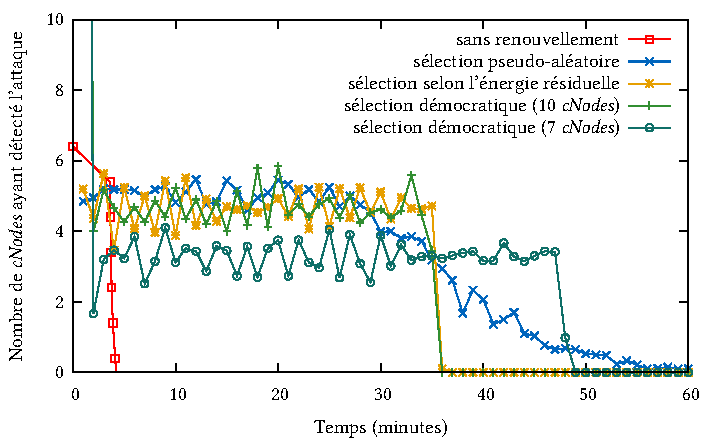
\includegraphics[height=.48\textheight]{Figs/plot_sd_detectionXtime-minute_20J.pdf}
  \end{minipage}
\end{frame}
%===============================================================================
\begin{frame}{Avantages et inconvénients}
  \scriptsize
  \begin{tabu}{X[1,c,m] X[2,j,m] X[2,j,m]}
    %\toprule
    \textsc{Méthode} & \centering \textsc{Avantages} & \centering \textsc{Inconvénients} \\
    %\midrule
    \toprule
    Aucun renouvellement
    & \textbullet\;Préservation des nœuds non sélectionnés
    & \textbullet\;Mauvaise surveillance
    \\
    \midrule
    Sélection aléatoire
    & \textbullet\;Consommation modérée\newline
    \textbullet\;Simple à mettre en œuvre\newline
    \textbullet\;Pourcentage constant de \cns\newline
    \textbullet\;Bonne rotation des \cns; processus aléatoire: pas d'attaques
    & \textbullet\;Équilibre moyen de la charge\newline
    \textbullet\;Risque: capteurs non couverts par les \cns sur certaines phases
    \\
    \midrule
    Sélection selon l'énergie résiduelle
    & \textbullet\;Bon équilibre de la charge\newline
    \textbullet\;Surveillance de tous les capteurs par au moins deux \cns
    & \textbullet\;\vns contraignants; couteux en énergie et lourds à implémenter\newline
    \textbullet\;Très gourmand en énergie
    \\
    \midrule
    Élection démocratique
    & \textbullet\;Bon équilibre de la charge\newline
    \textbullet\;Surveillance de tous les capteurs par $\ge$ 2~\cns\newline
    \textbullet\;Consommation modérée (après période initiale)\newline
    \textbullet\;Peut prendre en compte d'autres paramètres
    & \textbullet\;La période initiale consomme beaucoup d'énergie
    \\
    %\bottomrule
  \end{tabu}
\end{frame}
\begin{frame}{Recommandations}
  \small
  \begin{description}
    \item[Aucun renouvellement]\hfill\\Déconseillé, sauf si matériel dédié
    \item[Sélection aléatoire]\hfill\\Privilégie la longévité à la sécurité; perte de certains capteurs plus tôt que d'autres
    \item[Sélection selon l'énergie résiduelle]\hfill\\Préférer l'élection démocratique; sauf en cas de courtes périodes d'activité du cluster
    \item[Élection démocratique]\hfill\\Privilégie la sécurité; maintien aussi longtemps que possible de l'intégralité des capteurs en fonctionnement
  \end{description}
\end{frame}
%===============================================================================
\section{Modèles}
%===============================================================================
\begin{frame}{Différents modèles}
  Processus de détection et sélection aléatoire
  \newcounter{enb}
  \begin{enumerate}
    %\item Chaines de Markov à temps continu (CMTC)
    \item Réseaux de Petri (RPGSe)
    \item Logique stochastique (LSAH)
    \setcounter{enb}{\theenumi}
  \end{enumerate}

  \bigskip

  Interactions entre \cns et capteurs compromis
  \begin{enumerate}
    \setcounter{enumi}{\theenb}
    \item Jeux quantitatifs
  \end{enumerate}
\end{frame}
%%===============================================================================
%\subsection[CTMC]{Chaines de Markov à temps continu}
%%===============================================================================
%\begin{frame}{Chaines de Markov à temps continu}
  %\begin{itemize}
    %\item Ensemble de macro-états (un par \cn) composés de compteurs
    %\item Les compteurs sont implémentés à la réception de paquets des capteurs voisins
    %\item Transition pour vérifier s'il y a ou non détection d'un comportement suspect
    %\item Évaluation de certaines propriétés (probabilité de détection du capteur compromis…)
    %\item Au final, le modèle est assez peu adapté
  %\end{itemize}
%\end{frame}
%===============================================================================
\subsection[RPGSe]{Réseaux de Petri}
%===============================================================================
\begin{frame}{Réseaux de Petri}
  \alert{Réseaux de Petri stochastiques généralisés étendus} (RPSGe)
  \begin{itemize}
    \item utilisés pour modéliser des processus stochastiques
    \item transitions \alert{immédiates} ou \alert{minutées} (distribuées de façon exponentielle ou déterministe)
    \item arcs inhibiteurs
  \end{itemize}

  \vfill\centering
  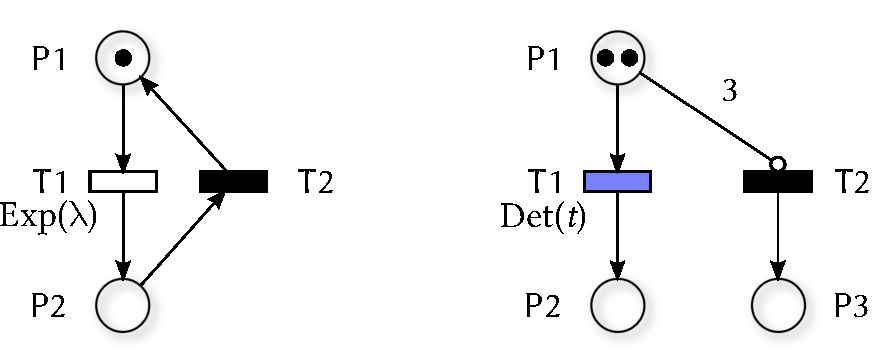
\includegraphics[height=.4\textheight]{Figs/RPSGe_example.pdf}
\end{frame}
%===============================================================================
\begin{frame}{RPGSe: briques de base}
  \centering
  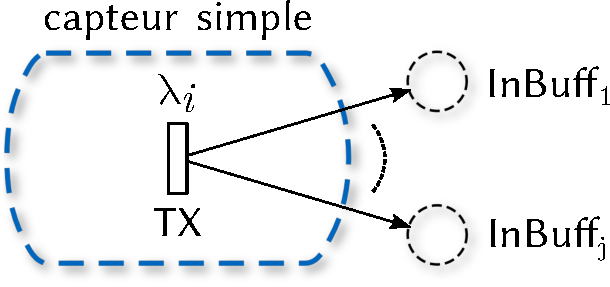
\includegraphics[height=.3\textheight]{Figs/RPSGe_sensing.pdf}
  \hfill
  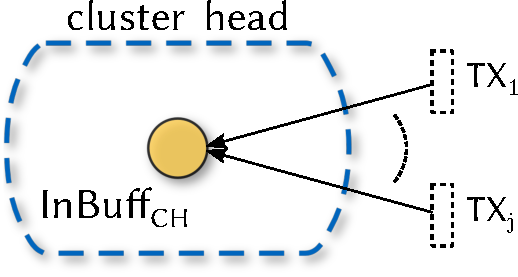
\includegraphics[height=.3\textheight]{Figs/RPSGe_CH.pdf}
  \vfill
  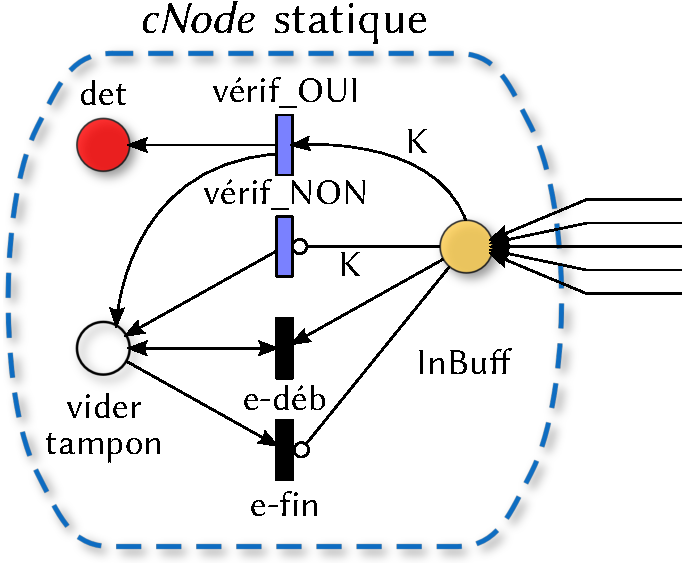
\includegraphics[height=.5\textheight]{Figs/RPSGe_cNode_static.pdf}
\end{frame}
\begin{frame}{RPGSe: Réseau sans renouvellement des \cns}
  \centering
  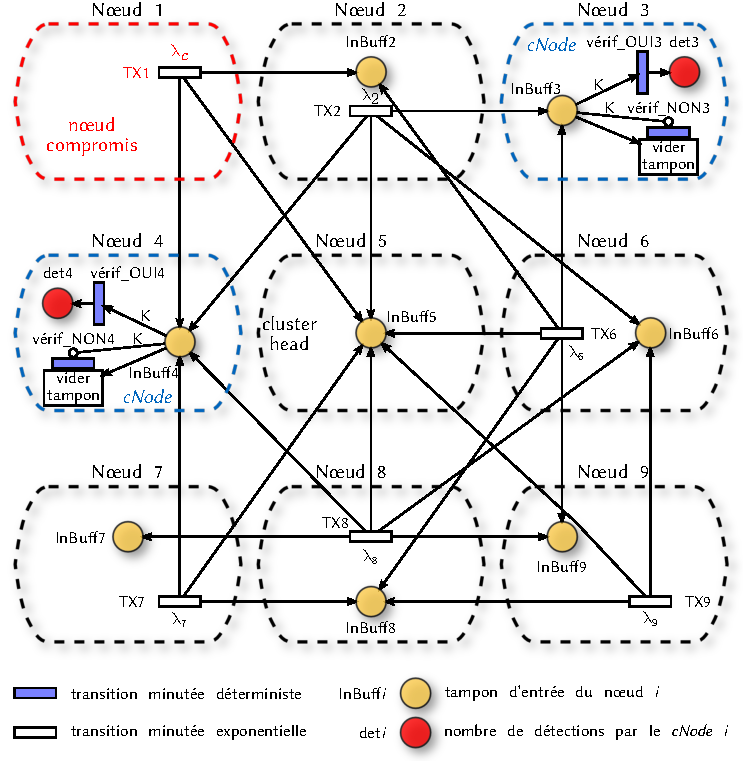
\includegraphics[height=.95\textheight]{Figs/RPSGe_network3x3_static.pdf}
\end{frame}
\begin{frame}{RPGSe: Capteurs complets}
  \centering
  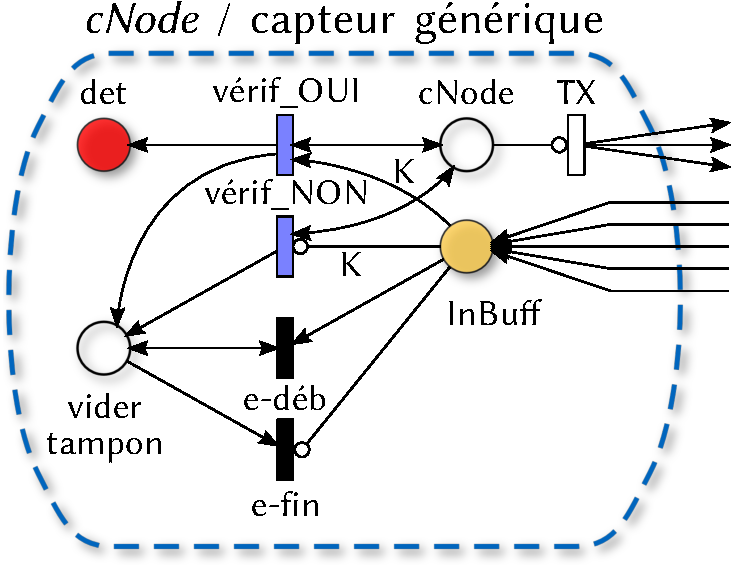
\includegraphics[height=.5\textheight]{Figs/RPSGe_cNode_generic.pdf}
\end{frame}
\begin{frame}{RPGSe: Réseau avec renouvellement des \cns}
  \centering
  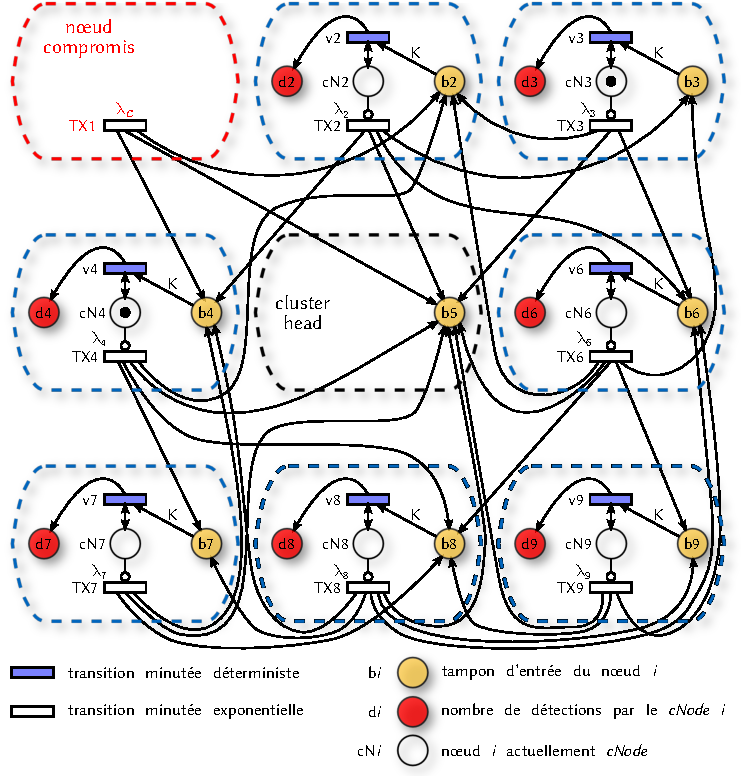
\includegraphics[height=.95\textheight]{Figs/RPSGe_network3x3_dynamic.pdf}
\end{frame}
%\begin{frame}{RPGSe: Processus de sélection}
  %\centering
  %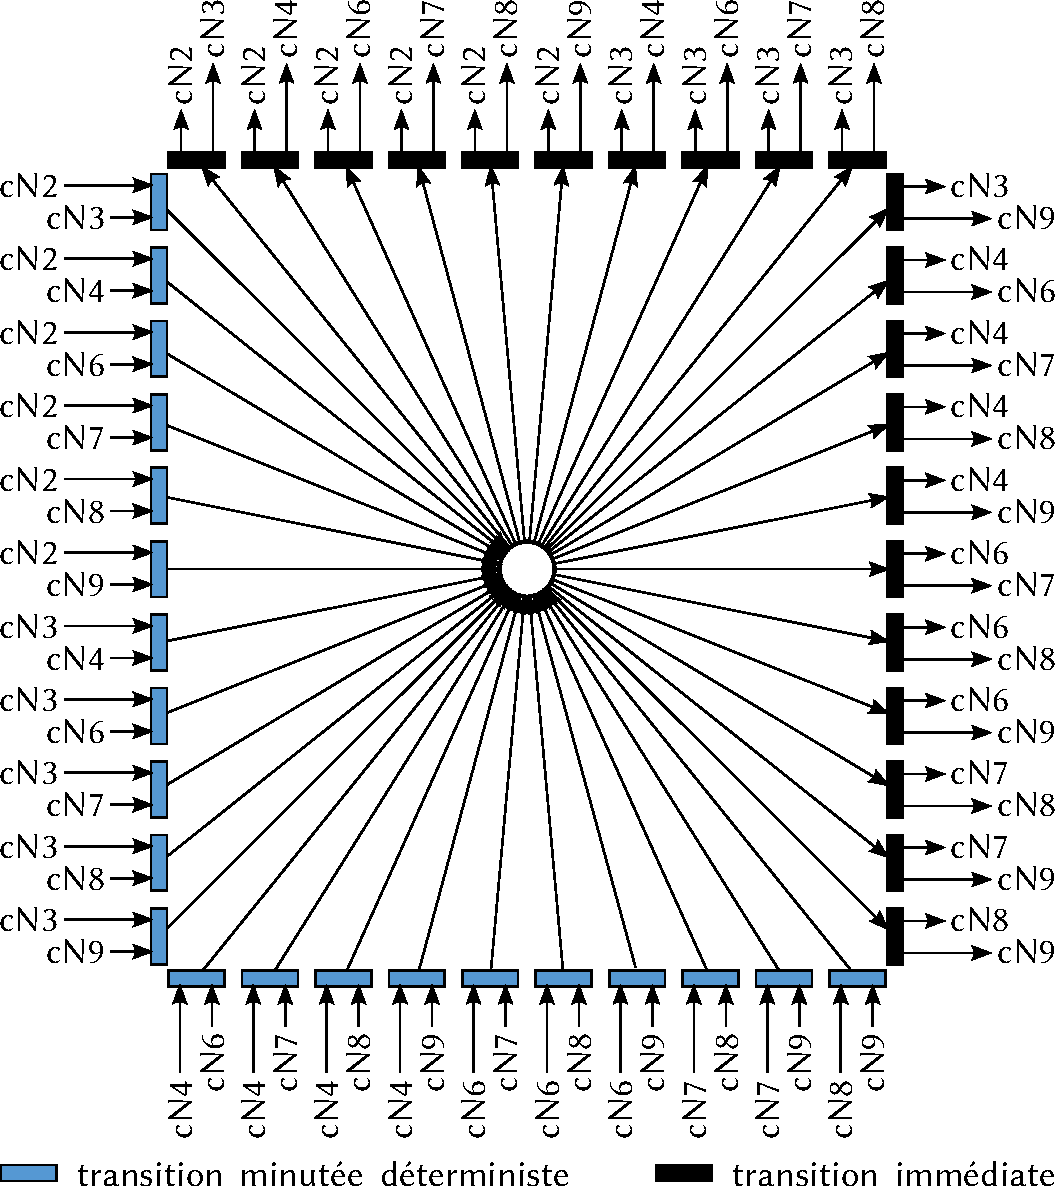
\includegraphics[height=.95\textheight]{Figs/RPSGe_network3x3_selection.pdf}
%\end{frame}
%===============================================================================
\subsection[LSAH]{Logique stochastique}
%===============================================================================
\begin{frame}{Logique stochastique avec automates hybrides}
  \begin{small}
    \begin{itemize}
      \item Basée sur un modèle RPSGe
      \item Mesures de performances exprimées en \alert{logique stochastique}
      \item Une formule de cette logique comprend:
        \begin{itemize}
          \item un \alert{automate linéaire hybride} (ALH)
          \item une \alert{expression} construite à partir des variables de l'ALH
        \end{itemize}
      \item Outils de \alert{\textit{model checking}} (COSMOS [\textsc{Ballarini} \textit{et al.}, 2011]) pour vérifier ces propriétés
    \end{itemize}
  \end{small}
  \begin{minipage}{.69\textwidth}
    \begin{tiny}
      \fbox{%
      \begin{tikzpicture}[auto, thick, >=stealth,scale=.5]
        \node[state, minimum width=7em, inner sep=-5em] (a) at (0,0) {%
          \hspace{.5em}
          \mbox{%
            \begin{tabular}{l @{}c @{\ }l}
              $\dot{x}_t$               & : & $1$\\
              $\dot{x}_{d_i}$           & : & $0$\\
              $\dot{x}_{\textit{bf}_i}$ & : & $M(\textit{bf}_i)$\\
              $\dot{x}_{\textsf{TX}_i}$ & : & $0$\\
            \end{tabular}%
          }
        };
        \node[state, minimum width=7em, accepting] (b) at (8,0) {};
        \draw[->] (a) edge[loop above, looseness=4] %
        node[] {$\textit{vrai}, \{\textsf{vérif\_OUI}_i\}, (x_{d_i}:=x_{d_i}+1)$} (a);
        \draw[->] (a) edge[loop below, looseness=4] %
        node[] {$\textit{vrai}, \{\textsf{TX}_i\}, (x_{\textsf{TX}_i}:=x_{\textsf{TX}_i}+1$)} (a);
        \draw[->] (a) edge[above] %
        node[] {$(x_t == T), \{\textit{tous}\}, \emptyset$} (b);
      \end{tikzpicture}%
    }
    \end{tiny}
  \end{minipage}
  \begin{minipage}{.30\textwidth}
    \begin{footnotesize}
      \raggedright
      Exemples d'expressions:\\
      \medskip
      $Z_1\equiv E(\mbox{dern}(x_{d_i}))$\\
      $Z_2\equiv E(\mbox{dern}(x_{d_i}+x_{d_{i'}}))$\\
      $Z_3\equiv E(\mbox{dern}(x_{\mathsf{TX}_i}))$\\
      $Z_4\equiv E(\mbox{int}(x_{\mathit{bf}_i}))$\\
    \end{footnotesize}
  \end{minipage}
\end{frame}
%===============================================================================
\subsection{Jeux quantitatifs}
%===============================================================================
\begin{frame}{Jeux quantitatifs}
  \small
  Principe:
  \begin{itemize}
    \item \alert{Formule de gain} à vérifier pour obtenir la victoire
    \item Problème de victoire: pour une configuration initiale et une formule de gain, existe-t-il une stratégie permettant d'obtenir la victoire?
    \item Problème du crédit initial: existe-t-il une valeur pour le crédit initial pour laquelle le problème de victoire a une réponse positive?
  \end{itemize}
  Plusieurs composantes pour les formules de gain: \alert{énergie et «\,gain\,»} (messages envoyés avec succès)
\end{frame}
\newcommand\idle         {\textsf{repos}\xspace}
\newcommand\listen       {\textsf{écoute}\xspace}
\newcommand\treatmsg     {\textsf{trait\_msg}\xspace}
\newcommand\treatnlmsg   {\textsf{trait}\\\textsf{msg}\xspace}
\newcommand\send         {\textsf{envoi}\xspace}
\newcommand\resend       {\textsf{renvoi}\xspace}
\newcommand\startsend    {\textsf{déb\_envoi}\xspace}
\newcommand\stopsend     {\textsf{fin\_envoi}\xspace}
\newcommand\startlisten  {\textsf{déb\_écoute}\xspace}
\newcommand\srlisten     {\textsf{déb\_éc.}\xspace}
\newcommand\stoplisten   {\textsf{fin\_écoute}\xspace}
\newcommand\startreceive {\textsf{déb\_réception}\xspace}
\newcommand\starttransmit{\textsf{déb\_retransmission}\xspace}
\newcommand\hold         {\textsf{attente}\xspace}
\newcommand\remainidle   {\textsf{cont\_repos}\xspace}
\newcommand\ignore       {\textsf{ignorer\_msg}\xspace}
\newcommand\gn           {{\ensuremath{\mathfrak{s}}}\xspace}
\newcommand\bn           {{\ensuremath{\mathfrak{c}}}\xspace}
\newcommand\chapterLACLbis{85,152,211}
\definecolor{chapterLACL}{RGB}{\chapterLACLbis}
\colorlet{SecTab}{chapterLACL!50}
\begin{frame}{Jeux quantitatifs --- graphes}
  \small
  Résultats:
  \begin{itemize}
    \item \alert{Cas général} indécidable
    \item \alert{Conjonction d'atomes}: possibilité de calculer une stratégie, potentiellement à mémoire infinie
    \item Dans ce dernier cas, possibilité de déterminer une \alert{approximation} avec mémoire finie
  \end{itemize}
  \vfill
  \begin{minipage}{0.48\textwidth}
    \centering
    % vim: se ft=tex:
\fontsize{4pt}{4pt}
\begin{tikzpicture}[%
    scale=.3, %
    state/.style={draw=none,circle,fill,blueLACL,text=white,circular drop shadow,minimum width=.5cm,align=center}, %
    edge/.style={->,>=stealth} %
  ]
  %\tikzset{state/.style={draw,circle,thick,minimum width=1cm,align=center}};

  \node[state] (ni) at (-3,+3) {\idle};
  \node[state] (nl) at (+3,+3) {\listen};
  \node[state] (nt) at (+3,-3) {\treatnlmsg};
  \node[state] (ns) at (-3,-3) {\send};

  % IDLE <-> LISTEN
  \draw[edge] (ni) to[bend left=20] node[above]{\startlisten: (-1,0)} (nl);
  \draw[edge] (nl) to[bend left=20] node[below]{\stoplisten: (0,0)} (ni);

  % IDLE <-> SEND
  \draw[edge] (ni) to[bend left=20] node[midway,below=.5cm,right=.1cm,rotate=90]{\startsend: (-2,+1)} (ns);
  \draw[edge] (ns) to[bend left=20] node[midway,above,rotate=90]{\stopsend: (0,0)} (ni);

  % TREAT->SEND
  \draw[edge] (nt) to[bend left=20] node[below]{\starttransmit: (-2,0)} (ns);

  % LISTEN->TREAT
  \draw[edge] (nl) to[bend left=20] node[midway,below,rotate=90]{\startreceive: (0,0)} (nt);

  % Loop edges
  \draw[edge] (ni) edge[loop,in=110,out=160,looseness=5] node[above=.15cm,right=-.5cm]{\remainidle: (+1,0)} (ni);
  \draw[edge] (ns) edge[loop,in=200,out=250,looseness=5] node[below=.15cm,right=-.3cm]{\resend: (-2,0)} (ns);
  \draw[edge] (nt) edge[loop,in=290,out=340,looseness=5] node[below=.15cm,left=-.15cm]{\hold: (0,0)} (nt);

  % Init edge
  \draw[edge] (-5.5,+3) to (ni);
\end{tikzpicture}
\normalsize
\\
    {\scriptsize Capteur légitime}
  \end{minipage}\hfill
  \begin{minipage}{0.48\textwidth}
    \centering
    % vim: se ft=tex:
\fontsize{4pt}{4pt}
\begin{tikzpicture}[%
    scale=.3, %
    state/.style={draw=none,circle,fill,blueLACL,text=white,circular drop shadow,minimum width=.5cm,align=center}, %
    edge/.style={->,>=stealth} %
  ]
  %\tikzset{state/.style={draw,circle,thick,minimum width=1cm,align=center}};

  \node[state] (ni) at (-3,+3) {\idle};
  \node[state] (nl) at (+3,+3) {\listen};
  \node[state] (nt) at (+3,-3) {\treatnlmsg};
  \node[state] (ns) at (-3,-3) {\send};

  % IDLE <-> LISTEN
  \draw[edge] (ni) to[bend left=20] node[above]{\startlisten: (-1,0)} (nl);
  \draw[edge] (nl) to[bend left=20] node[below]{\stoplisten: (0,0)} (ni);

  % IDLE <-> SEND
  \draw[edge] (ni) to[bend left=20] node[midway,below=.5cm,right=.1cm,rotate=90]{\startsend: (-2,+1)} (ns);
  \draw[edge] (ns) to[bend left=20] node[midway,above,rotate=90]{\stopsend: (0,0)} (ni);

  % TREAT->SEND
  \draw[edge] (nt) to[bend left=20] node[below]{\starttransmit: (-2,0)} (ns);

  % LISTEN->TREAT
  \draw[edge] (nl) to[bend left=20] node[midway,below,rotate=90]{\startreceive: (0,0)} (nt);

  % Loop edges
  \draw[edge] (ni) edge[loop,in=110,out=160,looseness=5] node[above=.15cm,right=-.5cm]{\remainidle: (+1,0)} (ni);
  \draw[edge] (ns) edge[loop,in=200,out=250,looseness=5] node[below=.15cm,right=-.3cm]{\resend: (-2,0)} (ns);
  \draw[edge] (nt) edge[loop,in=290,out=340,looseness=5] node[below=.15cm,left=-.15cm]{\hold: (0,0)} (nt);

  % Init edge
  \draw[edge] (-5.5,+3) to (ni);

  %%% Bad node %%%
  \draw[edge] (nt) to node[rotate=-45,below,near start]{\ignore: (0,0)} (ni);
  %\draw[edge] (nl) to node[rotate=45,below,near start]{s\_send: (-2,+1)} (ns);
\end{tikzpicture}
\normalsize
\\
    {\scriptsize Capteur compromis}
  \end{minipage}
\end{frame}
%===============================================================================
\section{Perspectives}
%===============================================================================
\begin{frame}{Conclusion et perspectives}
  Conclusions
  \begin{itemize}
    \item Détection: trois mécanismes de renouvellement des \cns
    \item Les résultats numériques indiquent une bonne répartition de la consommation
    \item Différents modèles pour représenter ces outils, en déduire des propriétés
  \end{itemize}
\end{frame}

\begin{frame}{Conclusion et perspectives}
  Travaux futurs
  \begin{itemize}
    \item Poursuivre l'étude du modèle de jeux quantitatifs
    \item Analyser les systèmes obtenus à l'aide d'outils de \textit{model-checking}
    \item Varier les modèles et les solutions, rechercher d'autres méthodes de renouvellement ou même de détection
    \item Confronter les mécanismes proposés à des applications réelles (plate-forme opérationnelle)
  \end{itemize}
  \vfill

  \uncover<2>{%
    \begin{exampleblock}{Merci beaucoup!}
      \center Questions
    \end{exampleblock}
  }
\end{frame}
%===============================================================================
%===============================================================================
\end{document}
